\documentclass[a4paper, 12pt]{article}
\usepackage[utf8]{inputenc}
\usepackage[english, russian]{babel}
\usepackage{latexsym}
\usepackage{amsmath}
\usepackage{amssymb}
\usepackage{graphicx}

\begin{document}
\title{Численное моделирование нестационарного течения газа с использованием неявных разностных схем}
\author{Земцов Сергей}
\date{410 группа}
\maketitle

\newpage
\tableofcontents
\newpage

\section{Постановкa дифференциальной задачи}

Нестационарное двумерное движение вязкого баротропного газа описывается системой уравнений
$$
\begin{array}{l}
\cfrac{\partial \rho}{\partial t} + \cfrac{\partial \rho u_1}{\partial x_1}+ \cfrac{\partial \rho u_2}{\partial x_2} = 0, \\
\cfrac{\partial \rho u_1}{\partial t} + \cfrac{\partial \rho u_1^2}{\partial x_1} + \cfrac{\partial \rho u_1 u_2}{\partial x_2} 
	+ \cfrac{\partial p}{\partial x_1} 
	= \mu \Big(\cfrac{4}{3}\cfrac{\partial^2 u_1}{\partial x_1^2} + \cfrac{\partial^2 u_1}{\partial x_2^2}
	+  \cfrac{1}{3}\cfrac{\partial^2 u_2}{\partial x_1\partial x_2} \Big) + \rho f_1, \\
\cfrac{\partial \rho u_2}{\partial t} + \cfrac{\partial \rho u_1 u_2}{\partial x_1} + \cfrac{\partial \rho u_2^2}{\partial x_2}
	+ \cfrac{\partial p}{\partial x_2} 
	= \mu \Big(\cfrac{1}{3}\cfrac{\partial^2 u_1}{\partial x_1\partial x_2} + \cfrac{\partial^2 u_2}{\partial x_1^2}
	+  \cfrac{4}{3}\cfrac{\partial^2 u_2}{\partial^2 x_2} \Big) + \rho f_2, \\
p = p (\rho),
\end{array}
$$
где $\mu$ - коэффициент вязкости газа (известная неотрицательная константа), $p$ - давление газа (известная функция), $f$ - вектор внешних сил
(также известная функция от переменных Эйлера, см. ниже).

Неизвестные функции: плотность $\rho$ и вектор скорости $u$ являются функциями переменных Эйлера 
\begin{gather*}
(t, x) \in Q = [0, T] \times \Omega.
\end{gather*}

Граничные условия для неизвестного решения: $\rho|_{\Gamma^-} = \rho_{\gamma} = 1,\quad u_1|_{\Gamma^-} = \omega \in \{0,1;\  1\},\quad \cfrac{\partial u_1}{\partial x_1}\Big|_{\Gamma^+} = 0$. На оставшейся границе компоненты скорости равны нулю, а функция плотности считается неизвестной.

Для решения задачи вводится равномерная сетка с шагом $h_x$ по оси X, $h_y$ по оси Y, $\tau$ по времени.

\section{Схема для $\log(\rho)$ с центральными разностями}
\label{scheme1}

Для автоматического обеспечения условия положительности функции плотности систему дифференциальных уравнений можно преобразовать к виду
\begin{align*}
& \cfrac{\partial g}{\partial t} + \frac{1}{2}\sum_{k=1}^{2}\Big(u_k\cfrac{\partial g}{\partial x_k}+
  \cfrac{\partial u_k g}{\partial x_k} + (2-g)\cfrac{\partial u_k}{\partial x_k}\Big) = f_0,\\
& \cfrac{\partial u_k}{\partial t} + \frac{1}{3}(u_k\cfrac{\partial u_k}{\partial x_k} + 
  \cfrac{\partial u_k^2}{\partial x_k})
  + \frac{1}{2}\sum_{m=1,m\neq k}^{2}\Big( u_m\cfrac{\partial u_k}{\partial x_m}+
  \cfrac{\partial u_m u_k}{\partial x_m} - u_k\cfrac{\partial u_m}{\partial x_m}\Big)
  + p’_{\rho } \cfrac{\partial g}{\partial x_k} = \\
& = \cfrac{\mu}{\rho}\Bigg( \frac{4}{3} \cfrac{\partial^2 u_k}{\partial x_k^2} + 
  \sum_{m=1,m\neq k}^{2}\Big( \cfrac{\partial^2 u_k}{\partial x_m^2} + 
  \frac{1}{3} \cfrac{\partial^2 u_m}{\partial x_k \partial x_m} \Big)\Bigg) + f_k,\ k = 1..s,\\
& p = p(\rho), \quad g = ln\ \rho.
\end{align*}

Сеточную функцию, разностное приближение для плотности $\rho$, обозначим H. Аналогично, разностные аналоги g и u обозначим через G и V. Для поиска численного решения задачи используется следующая разностная схема:
\begin{align*}
& G_t + 0.5 \sum_{k=1}^{2}\Big(V_k \hat G_{\stackrel{0}{x_k}} + (V_k \hat G)_{\stackrel{0}{x_k}} 
  + 2 (\hat V_k)_{\stackrel{0}{x_k}} - G(V_k)_{\stackrel{0}{x_k}} \Big) = f_0,\ x \in \Omega _{\bar h};\\
& G_t + 0.5 \Big((V_k \hat G)_{x_k} + 2 (\hat V_k)_{x_k} - G(V_k)_{x_k}\Big) -\\
& -0.5h_k \Big( (GV_k)_{x_k\bar x_k}^{+1_k} - 0.5(GV_k)_{x_k\bar x_k}^{+2_k}
  + (2-G)((V_k)_{x_k\bar x_k}^{+1_k} - 0.5 (V_k)_{x_k\bar x_k}^{+2_k})\Big) = \\
& \qquad = f_0, \qquad x \in \gamma_k^-, k = 1,\ 2;\\
& G_t + 0.5 \Big((V_k \hat G)_{\bar x_k} + 2 (\hat V_k)_{\bar x_k} - G(V_k)_{\bar x_k}\Big) +\\
& + 0.5h_k \Big( (GV_k)_{x_k\bar x_k}^{-1_k} - 0.5(GV_k)_{x_k\bar x_k}^{-2_k}
  + (2-G)((V_k)_{x_k\bar x_k}^{-1_k} - 0.5 (V_k)_{x_k\bar x_k}^{-2_k})\Big) = \\
& \qquad = f_0, \qquad x \in \gamma_k^+, k = 1,\ 2;\\
& (V_k)_t + \frac{1}{3}\Big( V_k(\hat V_k)_{\stackrel{0}{x_k}} + (V_k \hat V_k)_{\stackrel{0}{x_k}} \Big) +\\
& + \frac{1}{2}\sum_{m=1,m\neq k}^{2}\Big( 
  V_m(\hat V_k)_{\stackrel{0}{x_m}} + (V_m \hat V_k)_{\stackrel{0}{x_m}} - V_k(\hat V_m)_{\stackrel{0}{x_m}} \Big) +\\
& + p’_{\rho }(e^{G})\hat G_{\stackrel{0}{x_m}} = \tilde{\mu} \Bigg( \frac{4}{3}(\hat V_k)_{x_k\bar x_k}
  + \sum_{m=1,m\neq k}^{2}(\hat V_k)_{x_m\bar x_m} \Bigg) -\\
& - (\tilde{\mu} - \mu e^{-G}) \Bigg( \frac{4}{3}(V_k)_{x_k\bar x_k} + \sum_{m=1,m\neq k}^{2}(V_k)_{x_m\bar x_m}
  \Bigg) +\\
& + \cfrac{\mu e^{-G}}{3} \sum_{m=1,m\neq k}^{2}(V_m)_{\stackrel{0}{x_k} \stackrel{0}{x_m}} + f_k,\quad x\in \Omega_{\bar h};\\
& \hat V_k = 0, \qquad x \in \gamma_{\bar h}, \qquad k = 1,\ 2.
\end{align*}

Распишем уравнения схемы в поточечном виде и преобразуем их, приведя подобные слагаемые при неизвестных значениях с верхнего слоя. Получим:
\begin{align*}
& 4 G_{m_1,m_2}^{n+1}  -\frac{\tau}{h_x}  G_{m_1-1,m_2}^{n+1}(V1_{m_1,m_2}^n + V1_{m_1-1,m_2}^n) +\ \frac{\tau}{h_x} G_{m_1+1,m_2}^{n+1}(V1_{m_1,m_2}^n + V1_{m_1+1,m_2}^n)\\
& -\frac{\tau}{h_y} G_{m_1,m_2-1}^{n+1}(V2_{m_1,m_2}^n + V2_{m_1,m_2-1}^n)
 + \frac{\tau}{h_y} G_{m_1,m_2+1}^{n+1}(V2_{m_1,m_2}^n + V2_{m_1,m_2+1}^n)\\
& -\frac{2\tau}{h_x} V1_{m_1-1,m_2}^{n+1} + \frac{2\tau}{h_x} V1_{m_1+1,m_2}^{n+1}
-\frac{2\tau}{h_y} V2_{m_1,m_2-1}^{n+1} +\ \frac{2\tau}{h_y} V2_{m_1,m_2+1}^{n+1} = \\
& =\ 4 G_{m_1,m_2}^n + \tau G_{m_1,m_2}^n 
\Bigg(\cfrac{V1_{m_1+1,m_2}^n - V1_{m_1-1,m_2}^n}{h_x} +  \cfrac{V2_{m_1,m_2+1}^n - V2_{m_1,m_2-1}^n}{h_y}\Bigg) \\
& +\ 4\tau f_0, \qquad x\in \Omega _h
\end{align*}
\begin{align*}
& G_{0,m_2}^{n+1}(2 - \frac{\tau}{h_x}V1_{0,m_2}^n) + G_{1,m_2}^{n+1}\frac{\tau}{h_x}V1_{1,m_2}^n + \\
& + \frac{2\tau}{h_x}V1_{1,m_2}^{n+1} - \frac{2\tau}{h_x}V1_{0,m_2}^{n+1} = 
  2 G_{0,m_2}^n + \frac{\tau}{h_x} G_{0,m_2}^n (V1_{1,m_2}^n - V1_{0,m_2}^n) + 2\tau f_0 +\\
& + \frac{\tau}{h_x} \Big( G_{0,m_2}^n V1_{0,m_2}^n - 2.5 G_{1,m_2}^n V1_{1,m_2}^n 
  + 2 G_{2,m_2}^n V1_{2,m_2}^n - 0.5 G_{3,m_2}^n V1_{3,m_2}^n + \\
& + (2 - G_{0,m_2}^n)
  (V1_{0,m_2}^n - 2.5 V1_{1,m_2}^n + 2 V1_{2,m_2}^n - 0.5 V1_{3,m_2}^n) \Big), \qquad x \in \gamma_k^-
\end{align*}
\begin{align*}
& G_{M,m_2}^{n+1}(2 + \frac{\tau}{h_x}V1_{M,m_2}^n) - G_{M-1,m_2}^{n+1}\frac{\tau}{h_x}V1_{M-1,m_2}^n + \\
& + \frac{2\tau}{h_x}V1_{M,m_2}^{n+1} - \frac{2\tau}{h_x}V1_{M-1,m_2}^{n+1} = 
  2 G_{M,m_2}^n + \frac{\tau}{h_x} G_{M,m_2}^n (V1_{M,m_2}^n - V1_{M-1,m_2}^n) + 2\tau f_0 -\\
& - \frac{\tau}{h_x} \Big( G_{M,m_2}^n V1_{M,m_2}^n - 2.5 G_{M-1,m_2}^n V1_{M-1,m_2}^n 
  + 2 G_{M-2,m_2}^n V1_{M-2,m_2}^n - 0.5 G_{M-3,m_2}^n V1_{M-3,m_2}^n + \\
& + (2 - G_{M,m_2}^n)
  (V1_{M,m_2}^n - 2.5 V1_{M-1,m_2}^n + 2 V1_{M-2,m_2}^n - 0.5 V1_{M-3,m_2}^n) \Big), \qquad x \in \gamma_k^+
\end{align*}
\begin{align*}
& V1_{m_1,m_2}^{n+1}(6 + 4\tau \tilde{\mu}(\cfrac{4}{h_x^2} + \cfrac{3}{h_y^2})) +\\
& V1_{m_1-1,m_2}^{n+1}(-\frac{\tau}{h_x}(V1_{m_1,m_2}^n + V1_{m_1-1,m_2}^n) -\tilde{\mu}\cfrac{8\tau}{h_x^2}) +\\
& V1_{m_1+1,m_2}^{n+1}(\frac{\tau}{h_x}(V1_{m_1,m_2}^n + V1_{m_1+1,m_2}^n) -\tilde{\mu}\cfrac{8\tau}{h_x^2}) +\\
& V1_{m_1,m_2-1}^{n+1}(-\frac{3\tau}{2h_y}(V2_{m_1,m_2}^n + V2_{m_1,m_2-1}^n) -\tilde{\mu}\cfrac{6\tau}{h_y^2}) +\\
& V1_{m_1,m_2+1}^{n+1}(\frac{3\tau}{2h_y}(V2_{m_1,m_2}^n + V2_{m_1,m_2+1}^n) -\tilde{\mu}\cfrac{6\tau}{h_y^2}) -\\
& - 3\frac{\tau}{h_x} p’_{\rho} G_{m_1-1,m_2}^{n+1} + 3\frac{\tau}{h_x} p’_{\rho} G_{m_1+1,m_2}^{n+1} = \\
& =  6 V1_{m_1,m_2}^n + 6\tau f_1 + \frac{3\tau}{2h_y}V1_{m_1,m_2}^n (V2_{m_1,m_2+1}-V2_{m_1,m_2-1}) - \\
& - (\tilde{\mu} - \mu e^{-G}) 6 \tau 
  \big(\cfrac{4}{3h_x^2}(V1_{m_1+1,m_2}^n - 2V1_{m_1,m_2}^n + V1_{m_1-1,m_2}^n) +\\
&  +  \cfrac{1}{h_y^2}(V1_{m_1,m_2+1}^n - 2V1_{m_1,m_2}^n + V1_{m_1,m_2-1}^n)\big) +\\
& + \mu e^{-G} \cfrac{\tau}{2h_x h_y}
  (V2_{m_1+1,m_2+1}^n - V2_{m_1-1,m_2+1}^n - V2_{m_1+1,m_2-1}^n + V2_{m_1-1,m_2-1}^n), \\
& \tilde{\mu} = \mu || e^{-G} ||.
\end{align*}

\section{Тестирование на гладком решении}
Рассмотрим функции:
$$
	u_1 (t, x_1, x_2) = \sin(x_1) \sin(x_2) \exp^t \\
$$
$$
	u_2 (t, x_1, x_2) = \sin(x_1) \sin(x_2) \exp^{-t} \\
$$
$$
	\rho (t, x_1, x_2) = (\cos(x_1) + 1.5) (\cos(x_2) + 1.5) \exp^{t}
$$
Сделаем эти функции решением задачи, путем определения функций $f_0, f_1, f_2$.

\subsection{Тест №1}
Посмотрим на нормы отклонения решения новой задачи от известного ответа.
Параметры $\mu = 0.1$

\begin{center}
	$||G - g||_c$
	\begin{tabular}{|c|c|c|c|}
		\hline 
		N  M& 20& 40& 80\\ 
		\hline 
		20 & 2.226118e-001 & 2.229332e-001 & 2.227963e-001 \\ \hline 
		40 & 1.625185e-001 & 1.490928e-001 & 1.470278e-001 \\ \hline 
		80 & 1.183744e-001 & 9.780931e-002 & 9.399656e-002 \\ \hline 
		\hline 
	\end{tabular} 
\end{center} 
\begin{center}
	$||G - g||_{L2}$
	\begin{tabular}{|c|c|c|c|}
		\hline 
		N  M& 20& 40& 80\\ 
		\hline 
		20 & 7.881502e-001 & 7.760840e-001 & 7.732262e-001 \\ \hline 
		40 & 4.415166e-001 & 4.242142e-001 & 4.205404e-001 \\ \hline 
		80 & 2.506339e-001 & 2.275291e-001 & 2.231311e-001 \\ \hline 
		\hline 
	\end{tabular} 
\end{center} 
\begin{center}
	$||G - g||_{2}^1$
	\begin{tabular}{|c|c|c|c|}
		\hline 
		N  M& 20& 40& 80\\ 
		\hline 
		20 & 1.084773e+000 & 9.429816e-001 & 8.630577e-001 \\ \hline 
		40 & 8.963833e-001 & 6.988282e-001 & 5.777637e-001 \\ \hline 
		80 & 8.348985e-001 & 6.072825e-001 & 4.586836e-001 \\ \hline 
		\hline 
	\end{tabular} 
\end{center} 
\begin{center}
	$||V1 - u1||_c$
	\begin{tabular}{|c|c|c|c|}
		\hline 
		N  M& 20& 40& 80\\ 
		\hline 
		20 & 3.587106e-001 & 3.571893e-001 & 3.567833e-001 \\ \hline 
		40 & 2.256584e-001 & 2.184677e-001 & 2.163800e-001 \\ \hline 
		80 & 1.369765e-001 & 1.258933e-001 & 1.232229e-001 \\ \hline 
		\hline 
	\end{tabular} 
\end{center} 
\begin{center}
	$||V1 - u1||_{L2}$
	\begin{tabular}{|c|c|c|c|}
		\hline 
		N  M& 20& 40& 80\\ 
		\hline 
		20 & 1.134281e+000 & 1.140679e+000 & 1.141334e+000 \\ \hline 
		40 & 6.427172e-001 & 6.415121e-001 & 6.406866e-001 \\ \hline 
		80 & 3.519757e-001 & 3.443347e-001 & 3.429484e-001 \\ \hline 
		\hline 
	\end{tabular} 
\end{center} 
\begin{center}
	$||V1 - u1||_{2}^1$
	\begin{tabular}{|c|c|c|c|}
		\hline 
		N  M& 20& 40& 80\\ 
		\hline 
		20 & 3.280914e+000 & 2.436311e+000 & 1.895991e+000 \\ \hline 
		40 & 3.259879e+000 & 2.327238e+000 & 1.699085e+000 \\ \hline 
		80 & 3.289118e+000 & 2.316687e+000 & 1.647871e+000 \\ \hline 
		\hline 
	\end{tabular} 
\end{center} 
\begin{center}
	$||V2 - u2||_c$
	\begin{tabular}{|c|c|c|c|}
		\hline 
		N  M& 20& 40& 80\\ 
		\hline 
		20 & 1.371596e-001 & 1.369522e-001 & 1.368953e-001 \\ \hline 
		40 & 8.303557e-002 & 8.094133e-002 & 8.068471e-002 \\ \hline 
		80 & 4.801745e-002 & 4.463771e-002 & 4.431233e-002 \\ \hline 
		\hline 
	\end{tabular} 
\end{center} 
\begin{center}
	$||V2 - u2||_{L2}$
	\begin{tabular}{|c|c|c|c|}
		\hline 
		N  M& 20& 40& 80\\ 
		\hline 
		20 & 4.394355e-001 & 4.301333e-001 & 4.274454e-001 \\ \hline 
		40 & 2.549795e-001 & 2.423606e-001 & 2.393553e-001 \\ \hline 
		80 & 1.468379e-001 & 1.316099e-001 & 1.282802e-001 \\ \hline 
		\hline 
	\end{tabular} 
\end{center} 
\begin{center}
	$||V2 - u2||_{2}^1$
	\begin{tabular}{|c|c|c|c|}
		\hline 
		N  M& 20& 40& 80\\ 
		\hline 
		20 & 7.274666e-001 & 5.903824e-001 & 5.133909e-001 \\ \hline 
		40 & 5.846181e-001 & 4.389401e-001 & 3.513036e-001 \\ \hline 
		80 & 5.165372e-001 & 3.677427e-001 & 2.729441e-001 \\ \hline 
		\hline 
	\end{tabular} 
\end{center} 
\begin{center}
	TIME
	\begin{tabular}{|c|c|c|c|}
		\hline 
		N  M& 20& 40& 80\\ 
		\hline 
		20 & 1.052000e+000 & 2.323400e+001 & 7.398490e+002 \\ \hline 
		40 & 1.314000e+000 & 1.189100e+001 & 3.979780e+002 \\ \hline 
		80 & 2.237000e+000 & 1.377600e+001 & 1.624820e+002 \\ \hline 
		\hline 
	\end{tabular} 
\end{center} 

Также для $\mu$ = 0.001

\begin{center}
	$||G - g||_c$
	\begin{tabular}{|c|c|c|c|}
		\hline 
		N  M& 20& 40& 80\\ 
		\hline 
		20 & 2.295651e-001 & 2.296185e-001 & 2.295576e-001 \\ \hline 
		40 & 1.734755e-001 & 1.582878e-001 & 1.558701e-001 \\ \hline 
		80 & 1.294093e-001 & 1.058871e-001 & 1.014020e-001 \\ \hline 
		\hline 
	\end{tabular} 
\end{center} 
\begin{center}
	$||G - g||_{L2}$
	\begin{tabular}{|c|c|c|c|}
		\hline 
		N  M& 20& 40& 80\\ 
		\hline 
		20 & 8.093506e-001 & 7.970034e-001 & 7.940868e-001 \\ \hline 
		40 & 4.560944e-001 & 4.381071e-001 & 4.343242e-001 \\ \hline 
		80 & 2.609654e-001 & 2.362643e-001 & 2.316317e-001 \\ \hline 
		\hline 
	\end{tabular} 
\end{center} 
\begin{center}
	$||G - g||_{2}^1$
	\begin{tabular}{|c|c|c|c|}
		\hline 
		N  M& 20& 40& 80\\ 
		\hline 
		20 & 1.100853e+000 & 9.602130e-001 & 8.817495e-001 \\ \hline 
		40 & 9.064776e-001 & 7.080743e-001 & 5.882787e-001 \\ \hline 
		80 & 8.435808e-001 & 6.122108e-001 & 4.637969e-001 \\ \hline 
		\hline 
	\end{tabular} 
\end{center} 
\begin{center}
	$||V1 - u1||_c$
	\begin{tabular}{|c|c|c|c|}
		\hline 
		N  M& 20& 40& 80\\ 
		\hline 
		20 & 3.671916e-001 & 3.653109e-001 & 3.647147e-001 \\ \hline 
		40 & 2.335176e-001 & 2.258276e-001 & 2.236546e-001 \\ \hline 
		80 & 1.449530e-001 & 1.317125e-001 & 1.289101e-001 \\ \hline 
		\hline 
	\end{tabular} 
\end{center} 
\begin{center}
	$||V1 - u1||_{L2}$
	\begin{tabular}{|c|c|c|c|}
		\hline 
		N  M& 20& 40& 80\\ 
		\hline 
		20 & 1.175211e+000 & 1.180273e+000 & 1.180626e+000 \\ \hline 
		40 & 6.724330e-001 & 6.690932e-001 & 6.678500e-001 \\ \hline 
		80 & 3.722931e-001 & 3.617727e-001 & 3.598263e-001 \\ \hline 
		\hline 
	\end{tabular} 
\end{center} 
\begin{center}
	$||V1 - u1||_{2}^1$
	\begin{tabular}{|c|c|c|c|}
		\hline 
		N  M& 20& 40& 80\\ 
		\hline 
		20 & 3.285783e+000 & 2.448737e+000 & 1.915902e+000 \\ \hline 
		40 & 3.257332e+000 & 2.329246e+000 & 1.705743e+000 \\ \hline 
		80 & 3.283435e+000 & 2.314672e+000 & 1.648520e+000 \\ \hline 
		\hline 
	\end{tabular} 
\end{center} 
\begin{center}
	$||V2 - u2||_c$
	\begin{tabular}{|c|c|c|c|}
		\hline 
		N  M& 20& 40& 80\\ 
		\hline 
		20 & 1.486234e-001 & 1.483809e-001 & 1.484719e-001 \\ \hline 
		40 & 9.080801e-002 & 8.918637e-002 & 8.901185e-002 \\ \hline 
		80 & 5.265125e-002 & 4.970741e-002 & 4.947207e-002 \\ \hline 
		\hline 
	\end{tabular} 
\end{center} 
\begin{center}
	$||V2 - u2||_{L2}$
	\begin{tabular}{|c|c|c|c|}
		\hline 
		N  M& 20& 40& 80\\ 
		\hline 
		20 & 4.566881e-001 & 4.476253e-001 & 4.450511e-001 \\ \hline 
		40 & 2.665928e-001 & 2.540846e-001 & 2.511399e-001 \\ \hline 
		80 & 1.540339e-001 & 1.387124e-001 & 1.354231e-001 \\ \hline 
		\hline 
	\end{tabular} 
\end{center} 
\begin{center}
	$||V2 - u2||_{2}^1$
	\begin{tabular}{|c|c|c|c|}
		\hline 
		N  M& 20& 40& 80\\ 
		\hline 
		20 & 7.422675e-001 & 6.059374e-001 & 5.297091e-001 \\ \hline 
		40 & 5.925206e-001 & 4.476225e-001 & 3.608399e-001 \\ \hline 
		80 & 5.197034e-001 & 3.715334e-001 & 2.773302e-001 \\ \hline 
		\hline 
	\end{tabular} 
\end{center} 
\begin{center}
	TIME
	\begin{tabular}{|c|c|c|c|}
		\hline 
		N  M& 20& 40& 80\\ 
		\hline 
		20 & 1.061000e+000 & 2.376200e+001 & 7.503460e+002 \\ \hline 
		40 & 1.327000e+000 & 1.200800e+001 & 3.707330e+002 \\ \hline 
		80 & 2.211000e+000 & 1.397100e+001 & 1.627290e+002 \\ \hline 
		\hline 
	\end{tabular} 
\end{center} 

По данным таблицам можно видеть, что уменьшение вязкости немного ухудшает расчет.
Также по $L_2$ норме хорошо виднен порядок схемы $\tau + h^2$.

\section {Численные эксперименты}
Слева показаны графики для входной скорости 1, справа - 0.1
\begin{figure}[h]
		\begin{minipage}[h]{0.4\linewidth}
			\includegraphics[width=1\linewidth]{./img/01_1_1/G/0}
		\end{minipage}
		\hfill
		\begin{minipage}[h]{0.4\linewidth}
			\includegraphics[width=1\linewidth]{./img/01_1_01/G/0}
		\end{minipage}
\end{figure}

\begin{figure}[h]
	\begin{minipage}[h]{0.4\linewidth}
		\includegraphics[width=1\linewidth]{./img/01_1_1/V/0}
	\end{minipage}
	\hfill
	\begin{minipage}[h]{0.4\linewidth}
		\includegraphics[width=1\linewidth]{./img/01_1_01/V/0}
	\end{minipage}
\end{figure}

\begin{figure}[h]
		\begin{minipage}[h]{0.4\linewidth}
			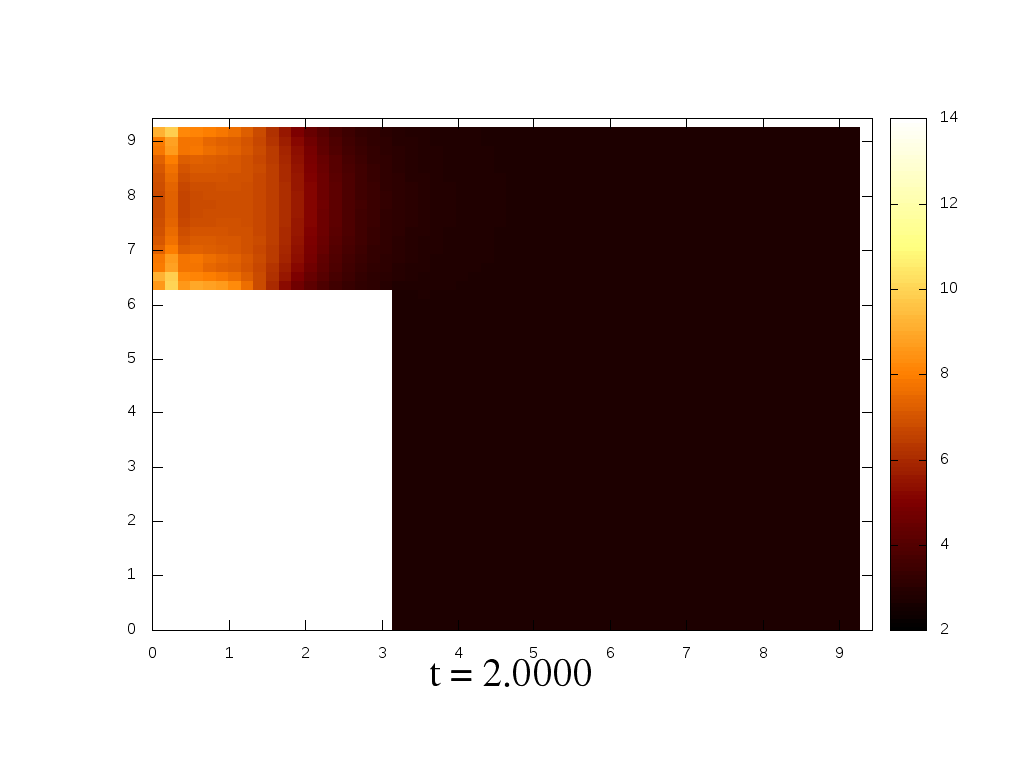
\includegraphics[width=1\linewidth]{./img/01_1_1/G/10}
		\end{minipage}
		\hfill
		\begin{minipage}[h]{0.4\linewidth}
			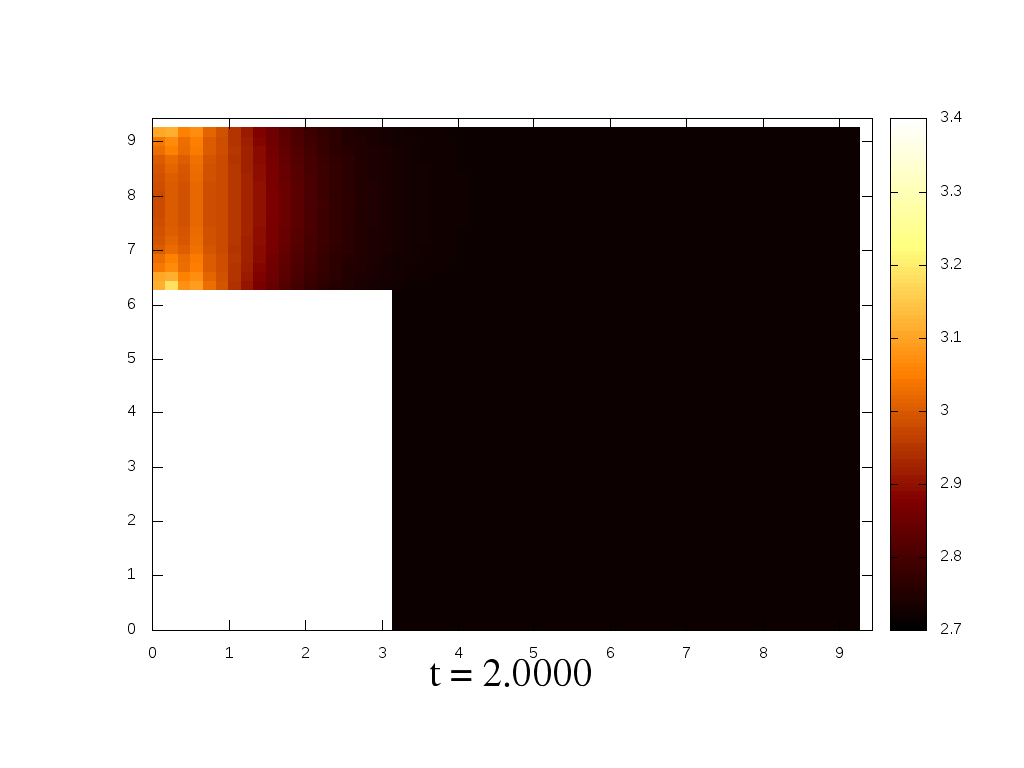
\includegraphics[width=1\linewidth]{./img/01_1_01/G/10}
		\end{minipage}
\end{figure}

\begin{figure}[h]
	\begin{minipage}[h]{0.4\linewidth}
		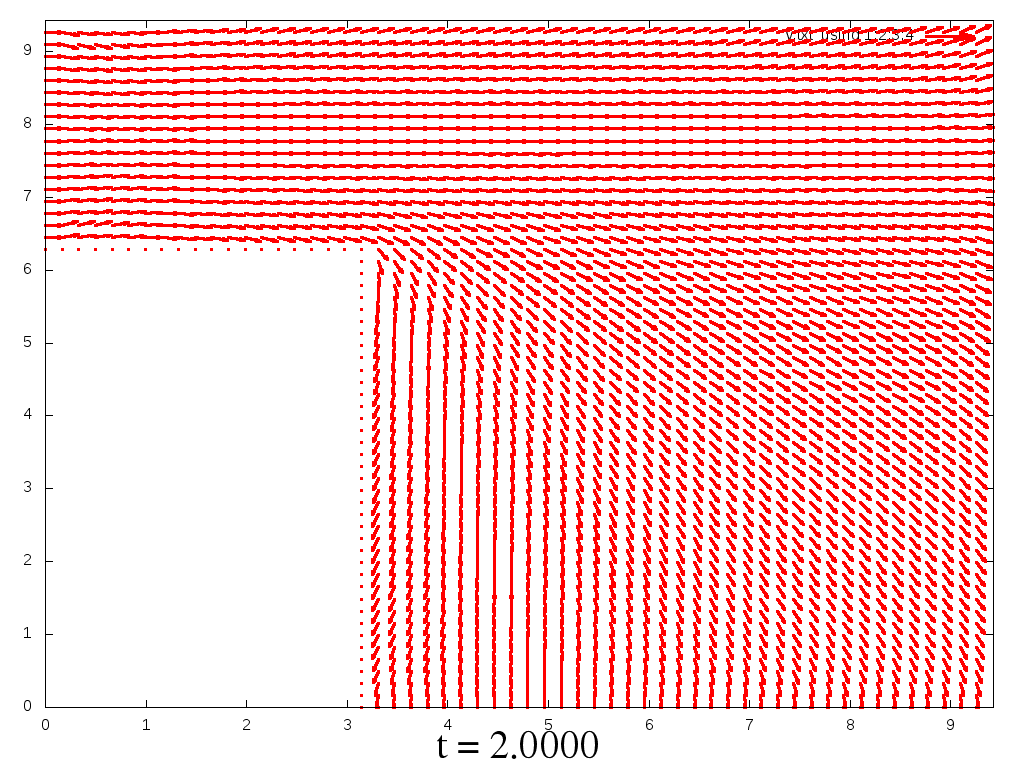
\includegraphics[width=1\linewidth]{./img/01_1_1/V/10}
	\end{minipage}
	\hfill
	\begin{minipage}[h]{0.4\linewidth}
		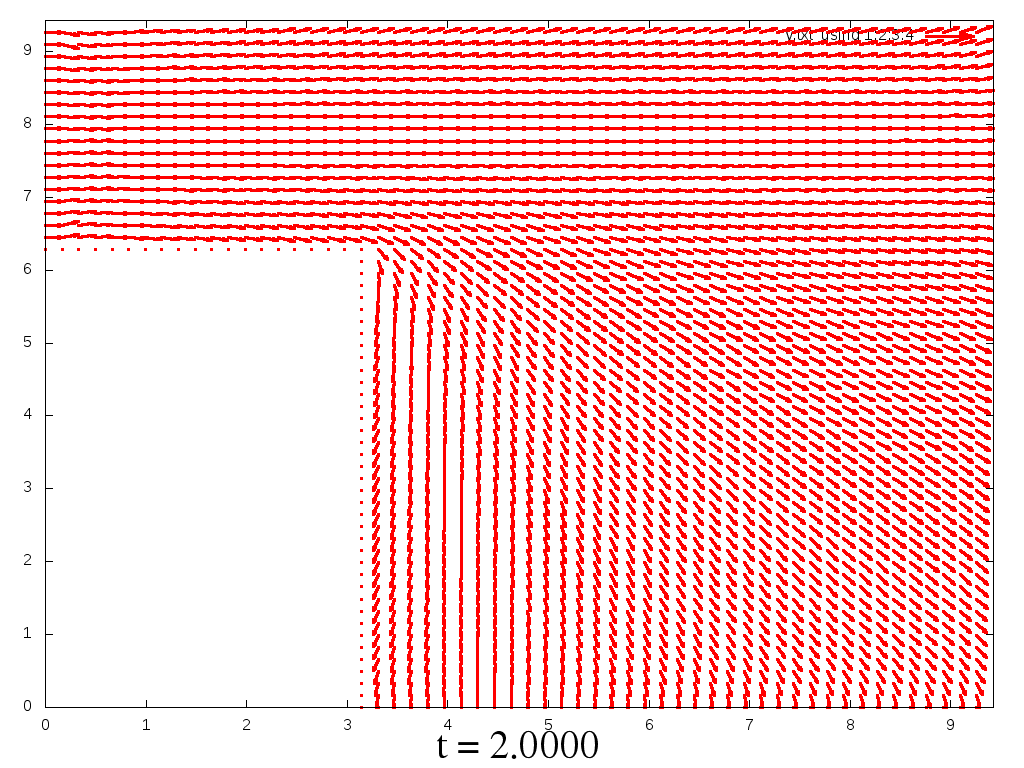
\includegraphics[width=1\linewidth]{./img/01_1_01/V/10}
	\end{minipage}
\end{figure}

\begin{figure}[h]
		\begin{minipage}[h]{0.4\linewidth}
			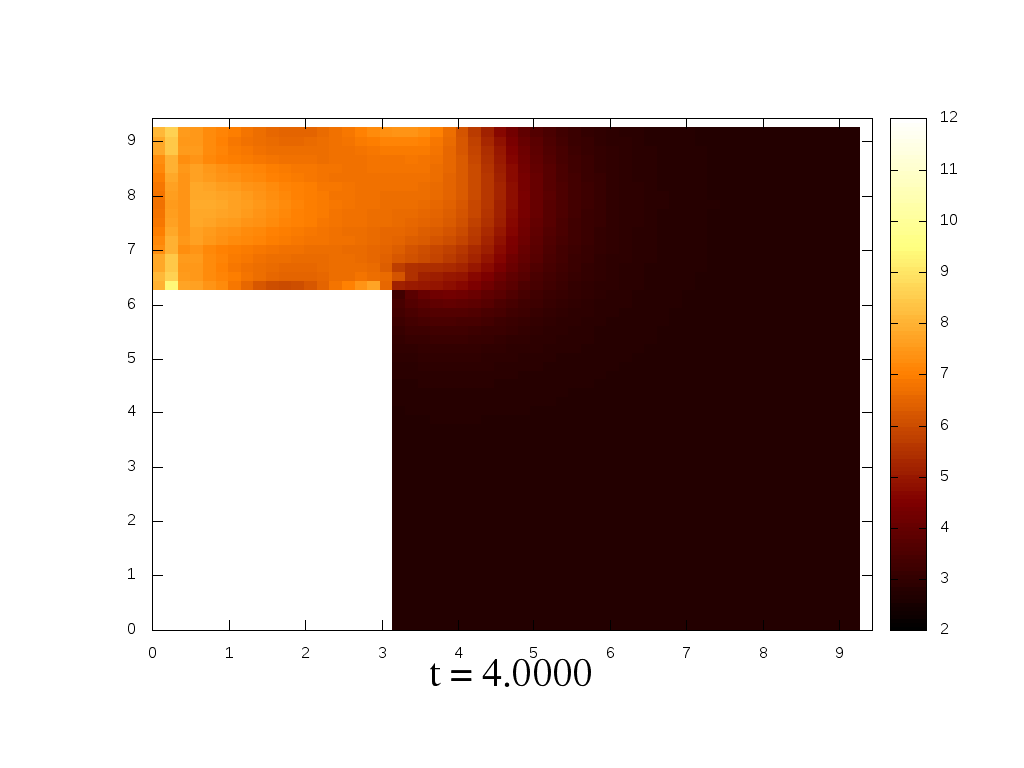
\includegraphics[width=1\linewidth]{./img/01_1_1/G/20}
		\end{minipage}
		\hfill
		\begin{minipage}[h]{0.4\linewidth}
			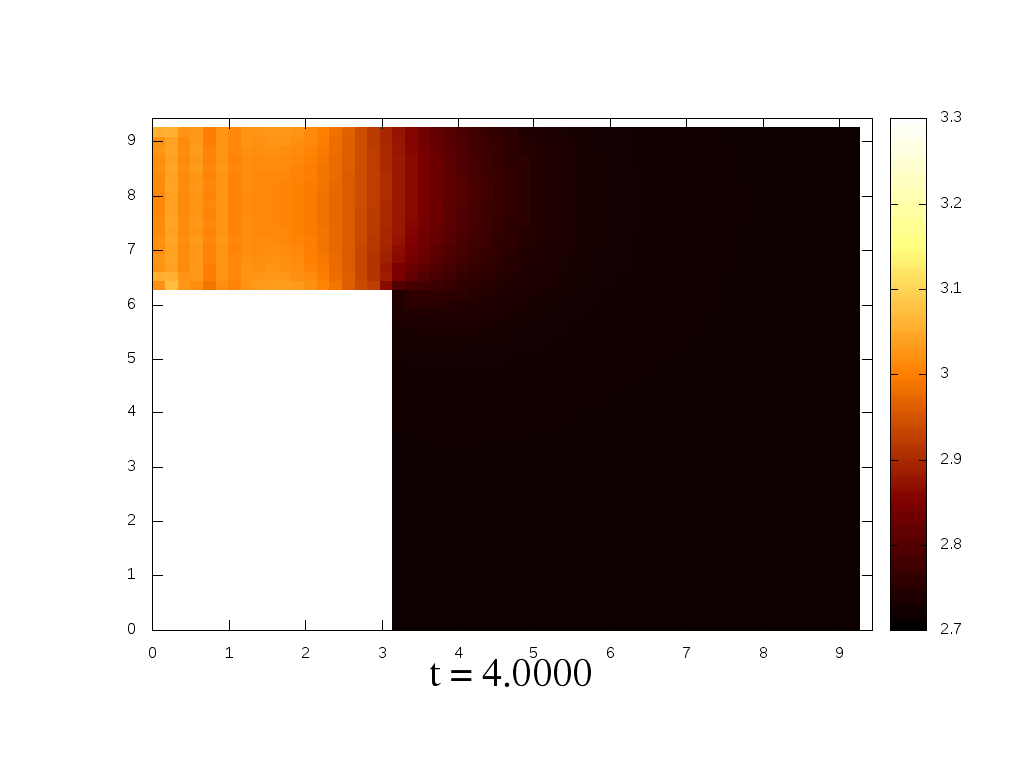
\includegraphics[width=1\linewidth]{./img/01_1_01/G/20}
		\end{minipage}
\end{figure}

\begin{figure}[h]
	\begin{minipage}[h]{0.4\linewidth}
		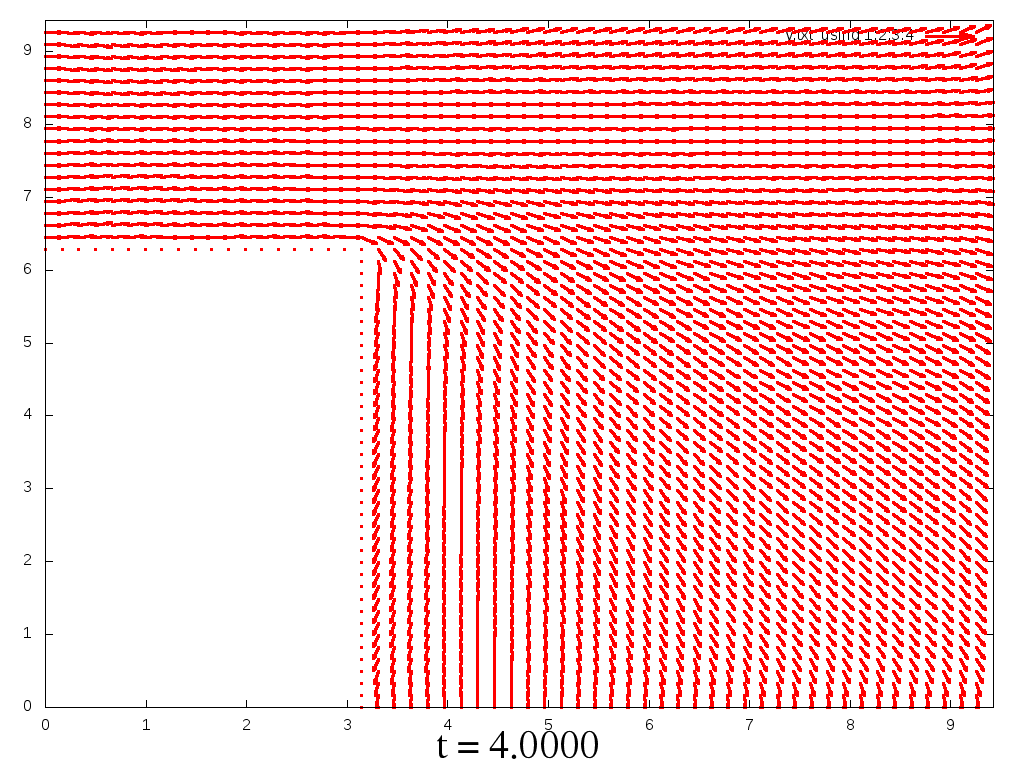
\includegraphics[width=1\linewidth]{./img/01_1_1/V/20}
	\end{minipage}
	\hfill
	\begin{minipage}[h]{0.4\linewidth}
		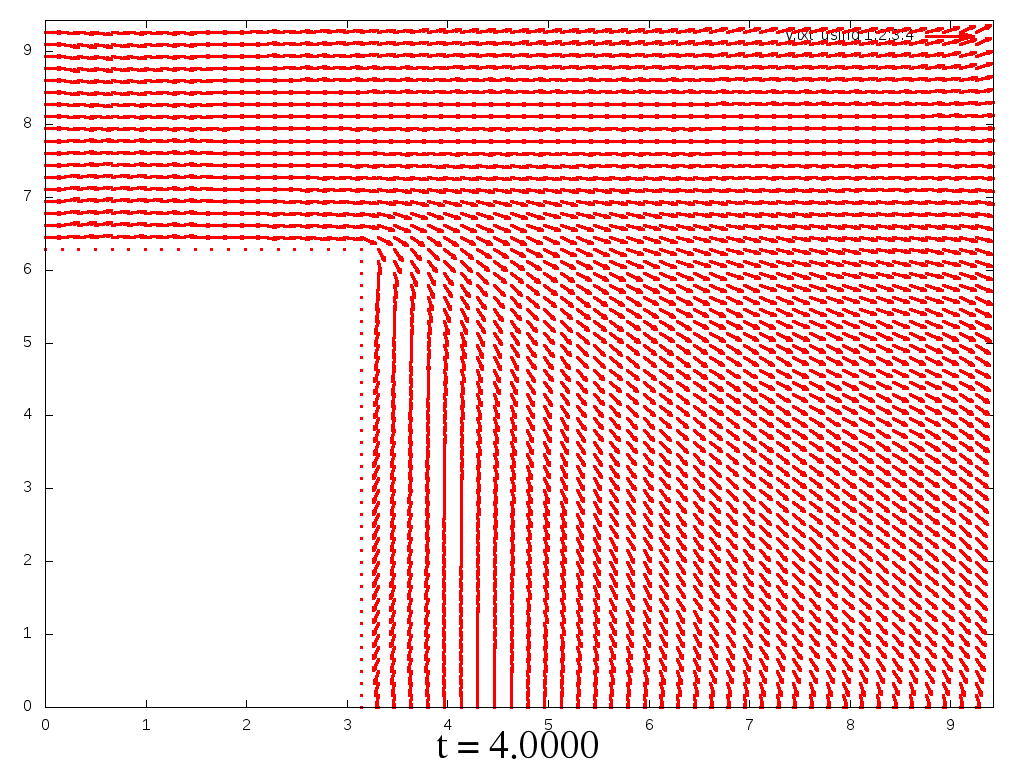
\includegraphics[width=1\linewidth]{./img/01_1_01/V/20}
	\end{minipage}
\end{figure}

\begin{figure}[h]
		\begin{minipage}[h]{0.4\linewidth}
			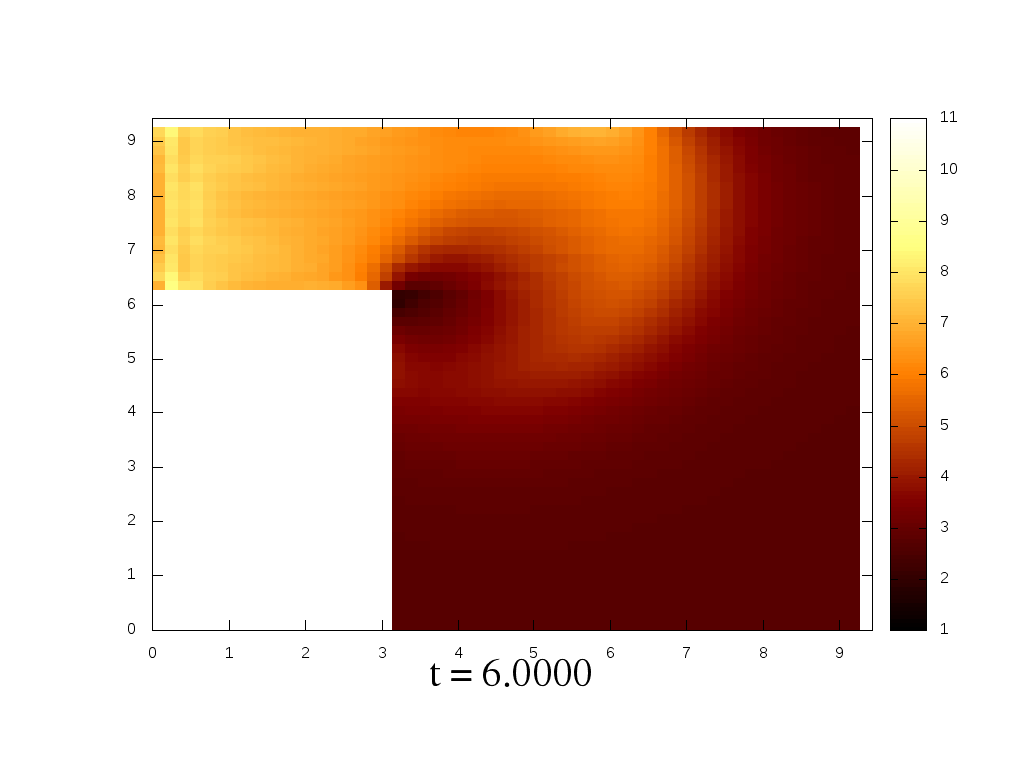
\includegraphics[width=1\linewidth]{./img/01_1_1/G/30}
		\end{minipage}
		\hfill
		\begin{minipage}[h]{0.4\linewidth}
			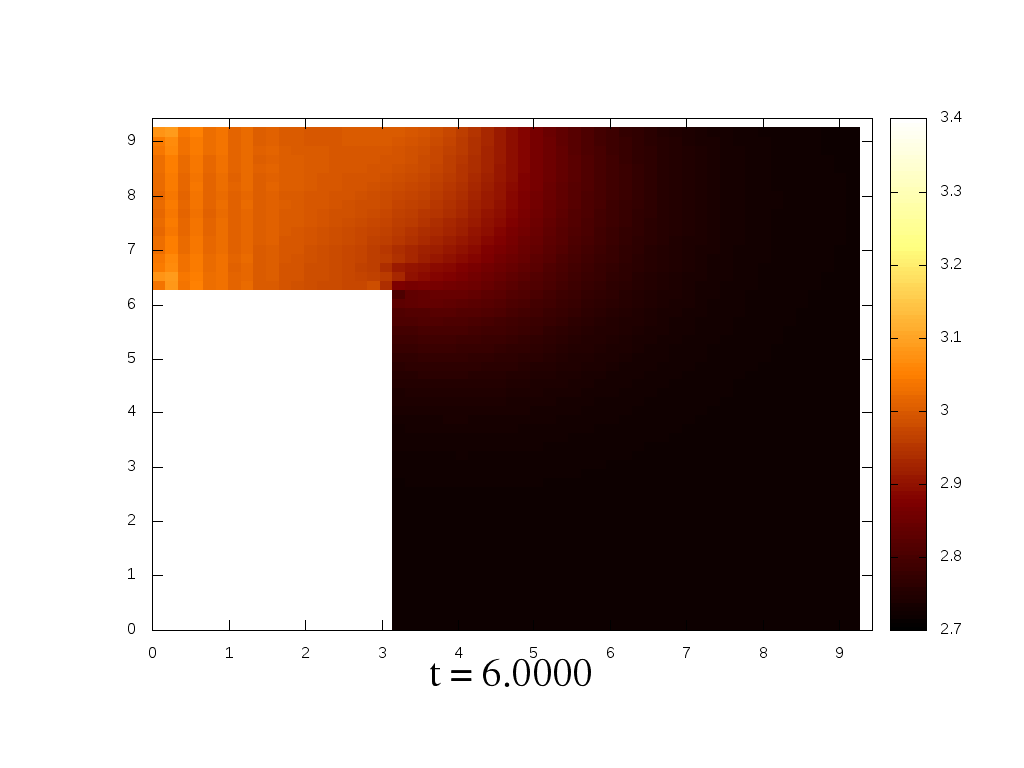
\includegraphics[width=1\linewidth]{./img/01_1_01/G/30}
		\end{minipage}
\end{figure}

\begin{figure}[h]
	\begin{minipage}[h]{0.4\linewidth}
		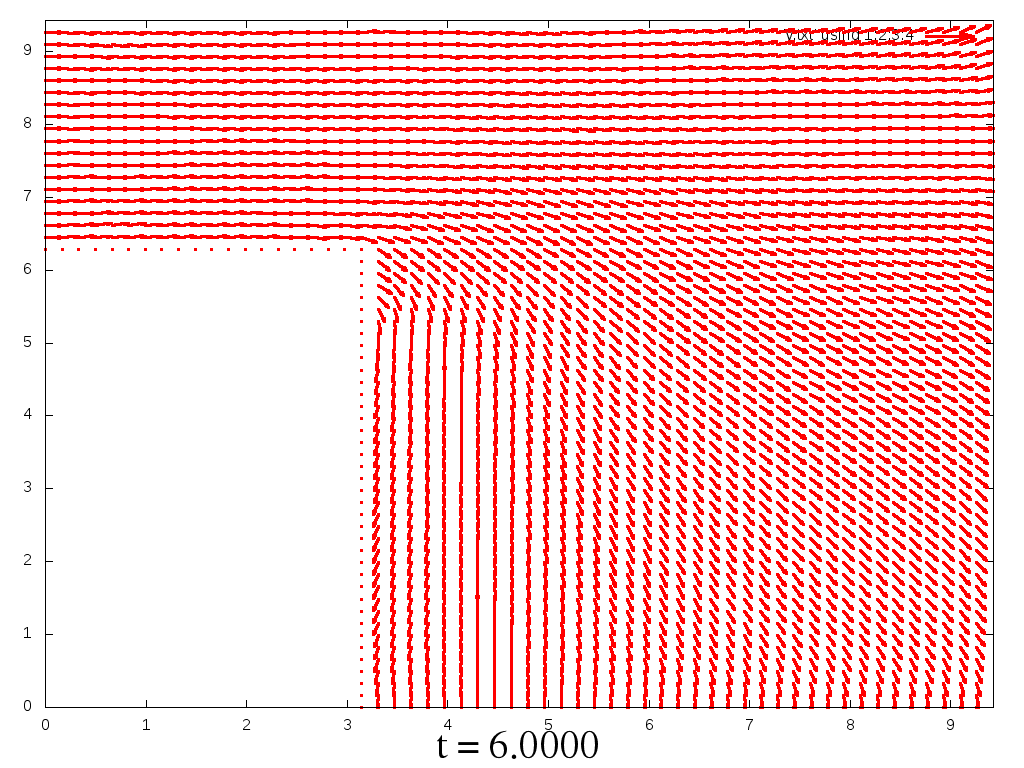
\includegraphics[width=1\linewidth]{./img/01_1_1/V/30}
	\end{minipage}
	\hfill
	\begin{minipage}[h]{0.4\linewidth}
		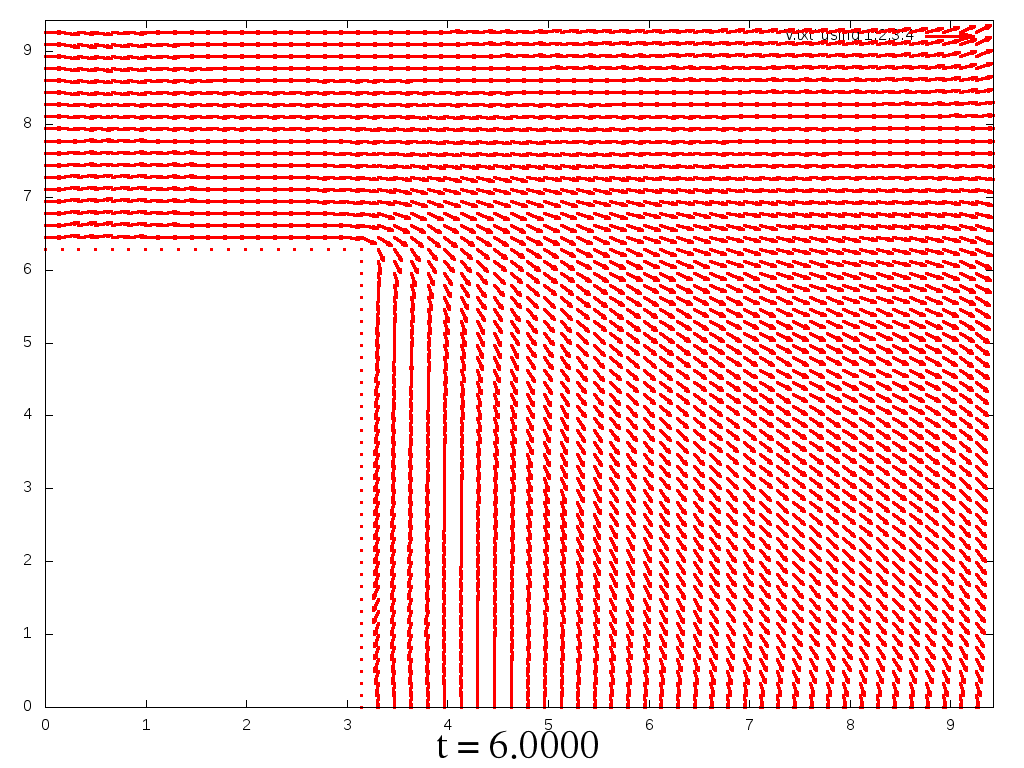
\includegraphics[width=1\linewidth]{./img/01_1_01/V/30}
	\end{minipage}
\end{figure}

\begin{figure}[h]
\begin{minipage}[h]{0.4\linewidth}
	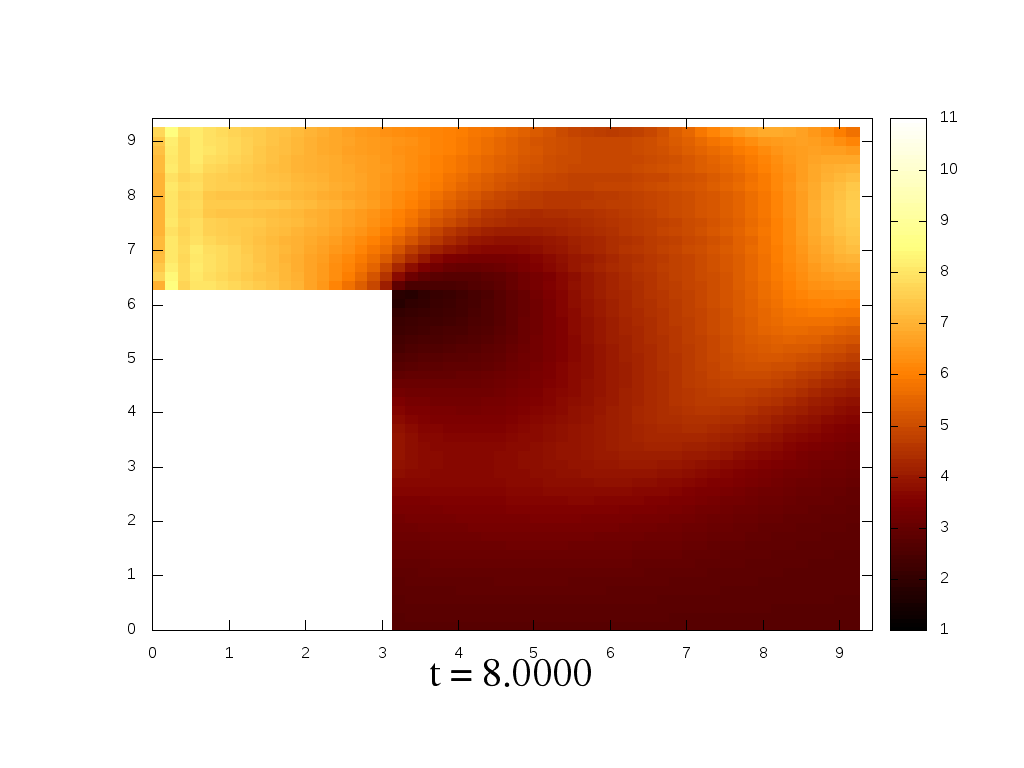
\includegraphics[width=1\linewidth]{./img/01_1_1/G/40}
\end{minipage}
\hfill
\begin{minipage}[h]{0.4\linewidth}
	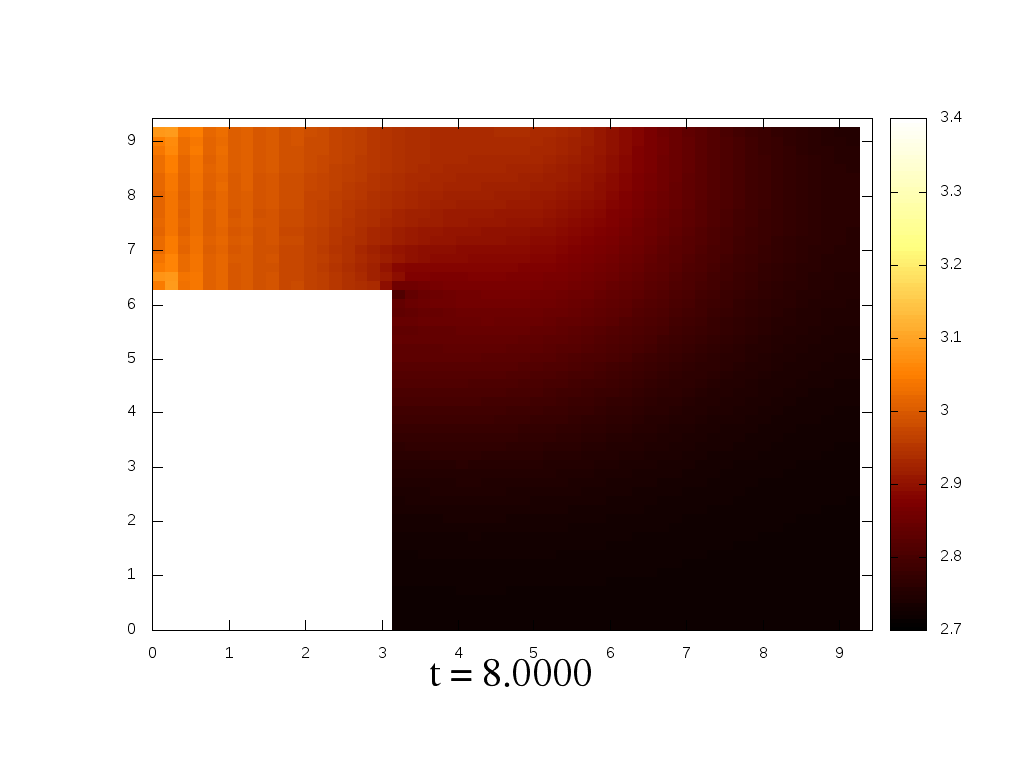
\includegraphics[width=1\linewidth]{./img/01_1_01/G/40}
\end{minipage}
\end{figure}

\begin{figure}[h]
	\begin{minipage}[h]{0.4\linewidth}
		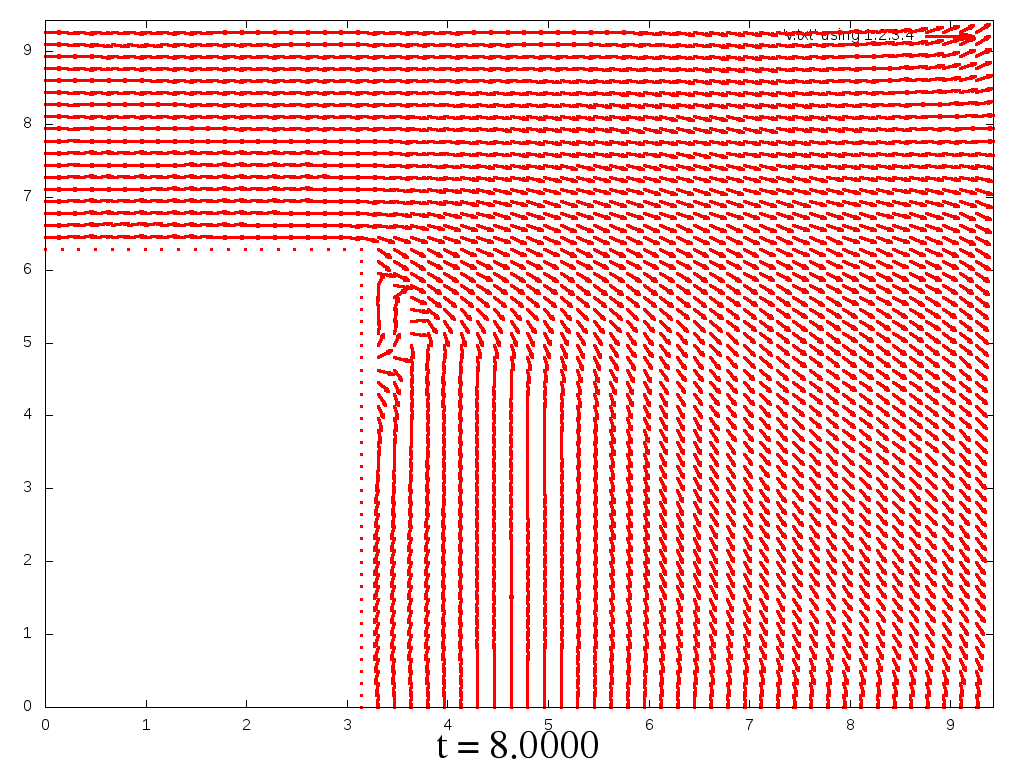
\includegraphics[width=1\linewidth]{./img/01_1_1/V/40}
	\end{minipage}
	\hfill
	\begin{minipage}[h]{0.4\linewidth}
		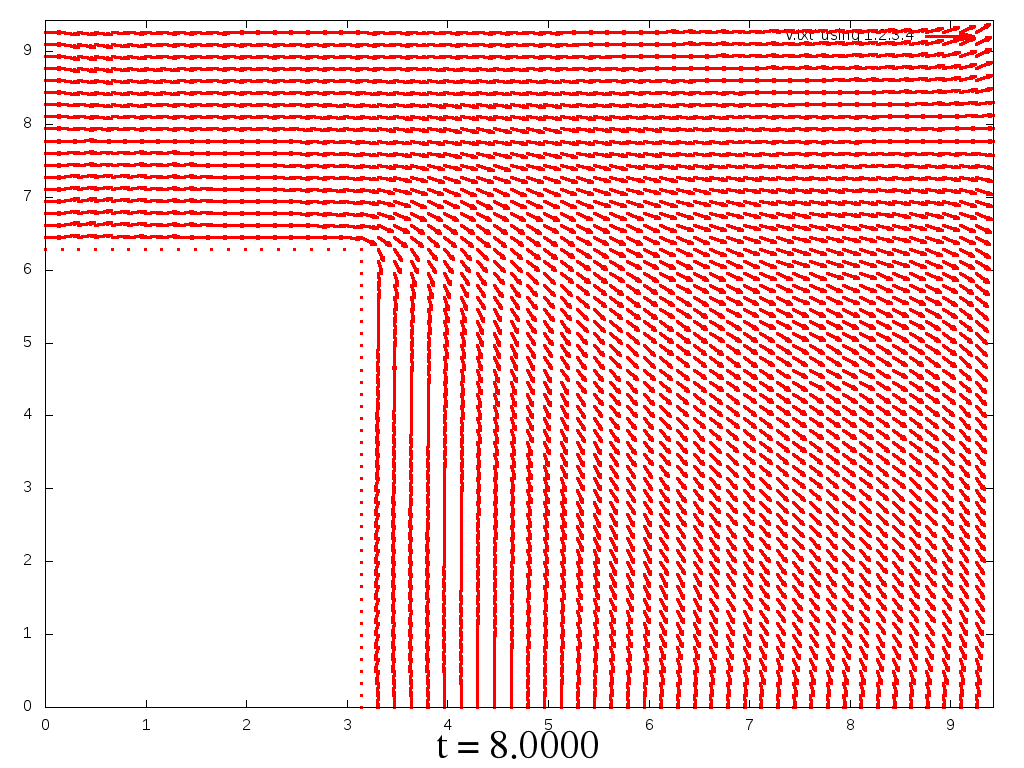
\includegraphics[width=1\linewidth]{./img/01_1_01/V/40}
	\end{minipage}
\end{figure}

\begin{figure}[h]
	\begin{minipage}[h]{0.4\linewidth}
		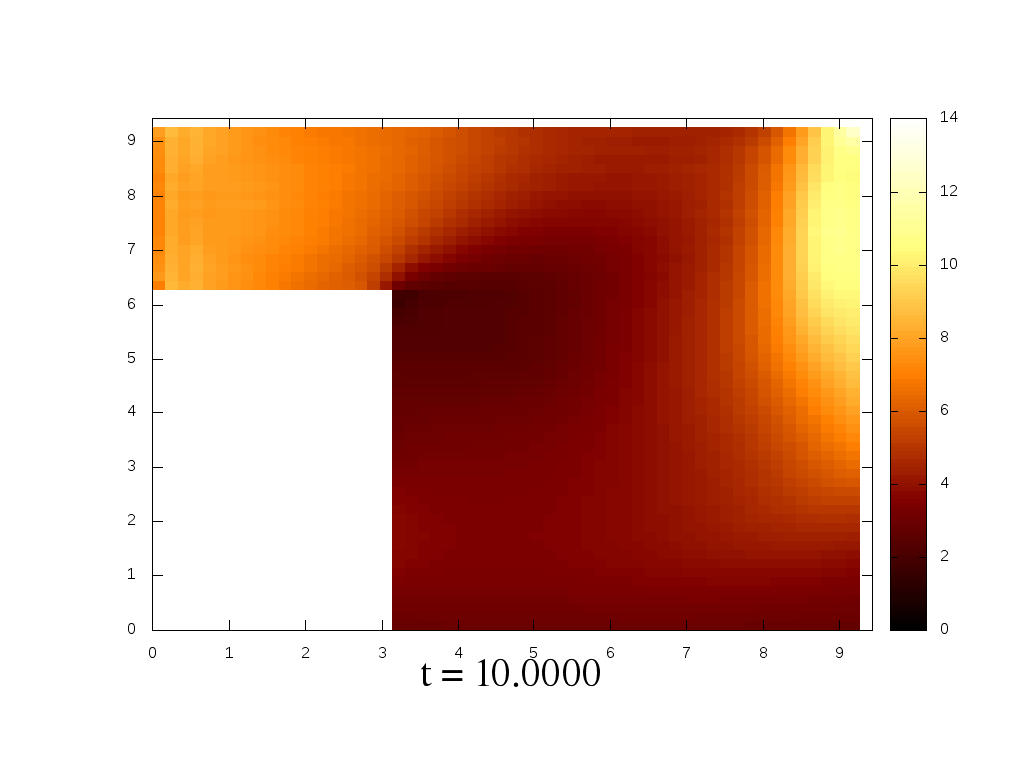
\includegraphics[width=1\linewidth]{./img/01_1_1/G/50}
	\end{minipage}
	\hfill
	\begin{minipage}[h]{0.4\linewidth}
		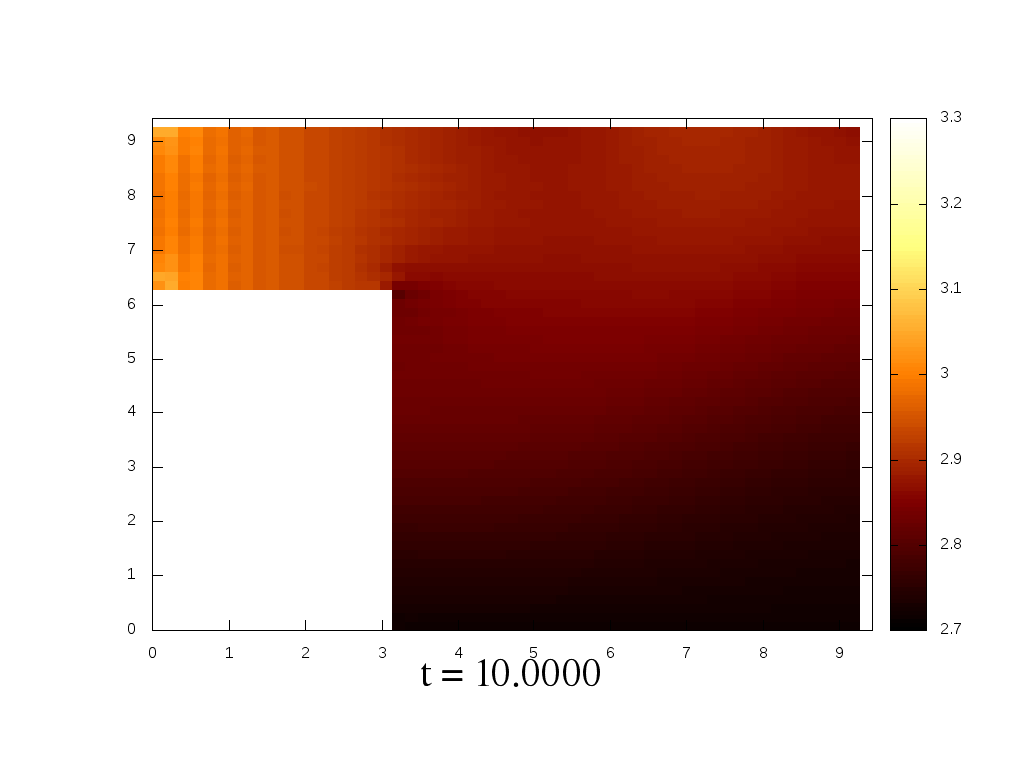
\includegraphics[width=1\linewidth]{./img/01_1_01/G/50}
	\end{minipage}
\end{figure}

\begin{figure}[h]
	\begin{minipage}[h]{0.4\linewidth}
		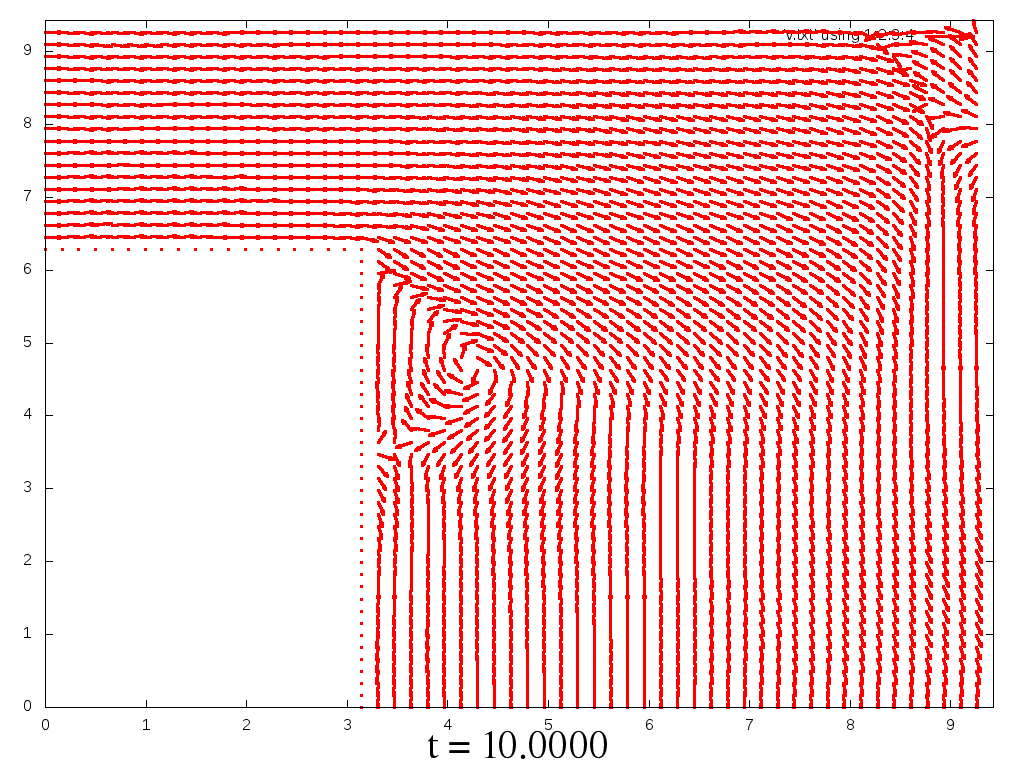
\includegraphics[width=1\linewidth]{./img/01_1_1/V/50}
	\end{minipage}
	\hfill
	\begin{minipage}[h]{0.4\linewidth}
		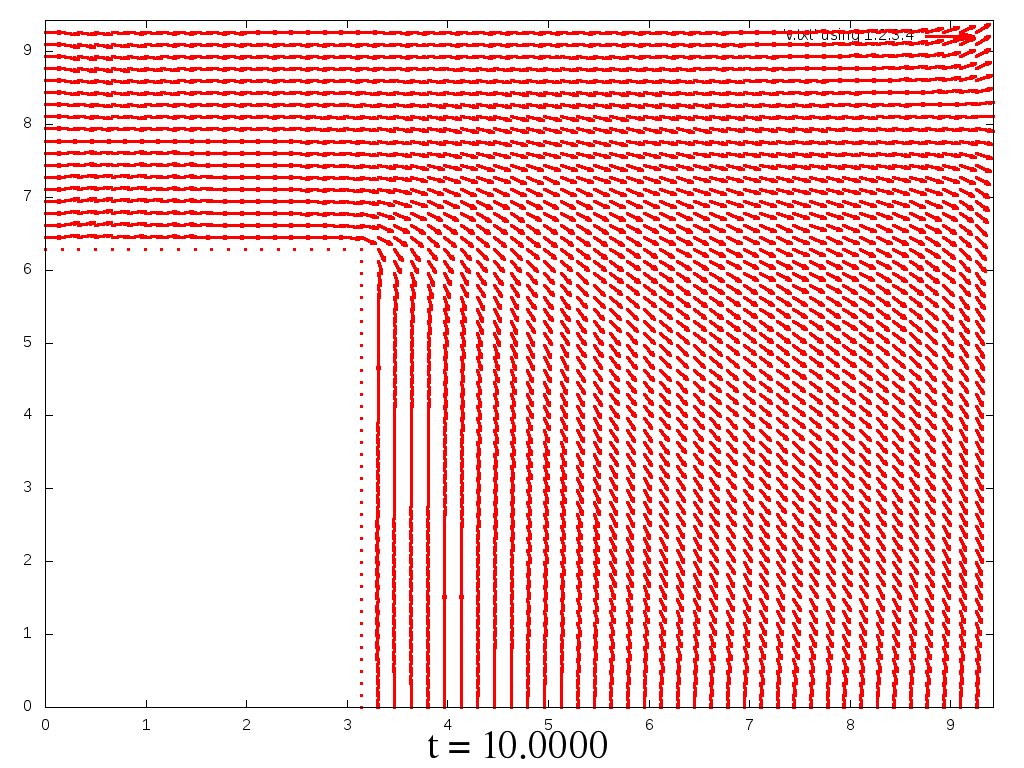
\includegraphics[width=1\linewidth]{./img/01_1_01/V/50}
	\end{minipage}
\end{figure}

\begin{figure}[h]
	\begin{minipage}[h]{0.4\linewidth}
		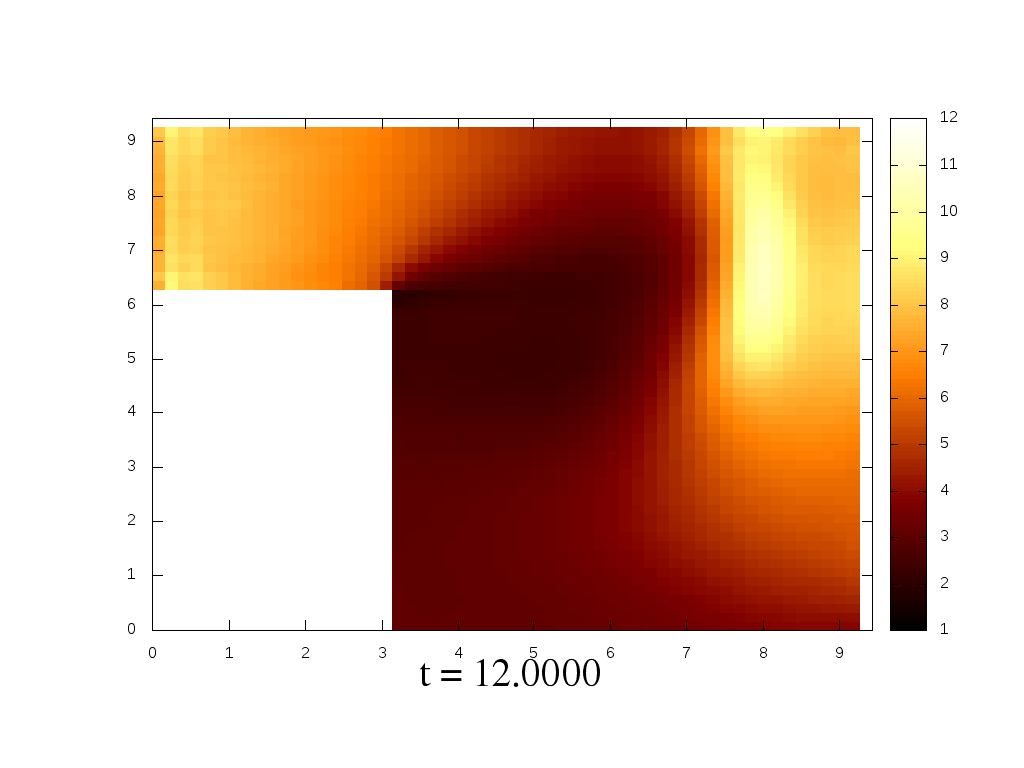
\includegraphics[width=1\linewidth]{./img/01_1_1/G/60}
	\end{minipage}
	\hfill
	\begin{minipage}[h]{0.4\linewidth}
		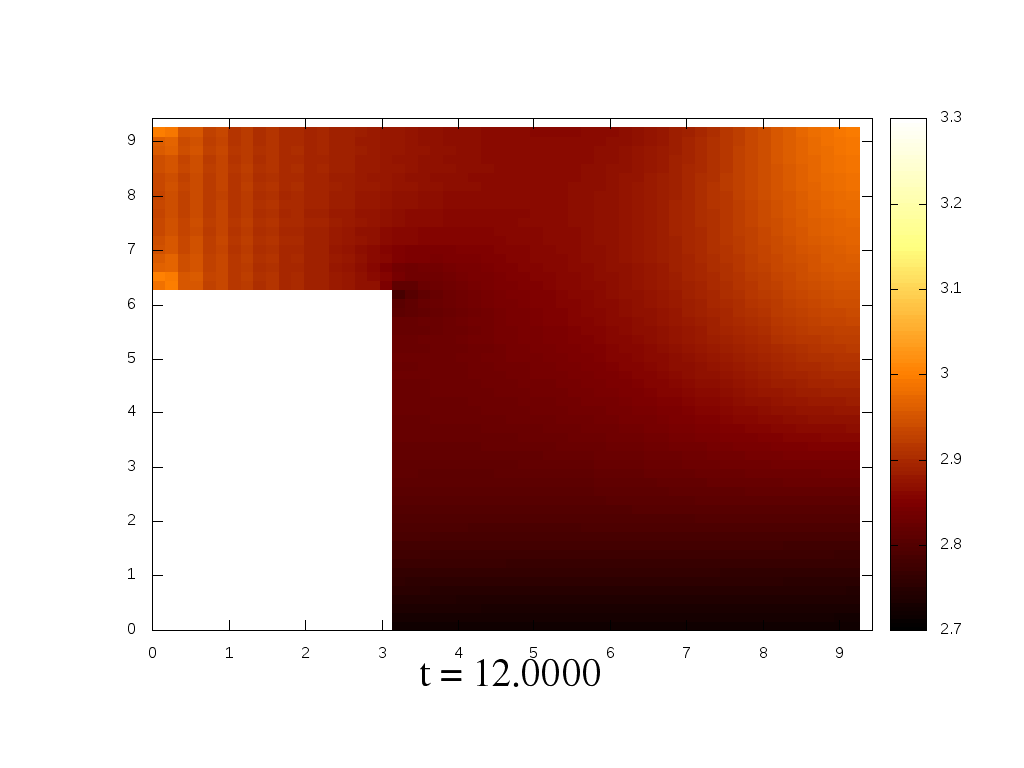
\includegraphics[width=1\linewidth]{./img/01_1_01/G/60}
	\end{minipage}
\end{figure}

\begin{figure}[h]
	\begin{minipage}[h]{0.4\linewidth}
		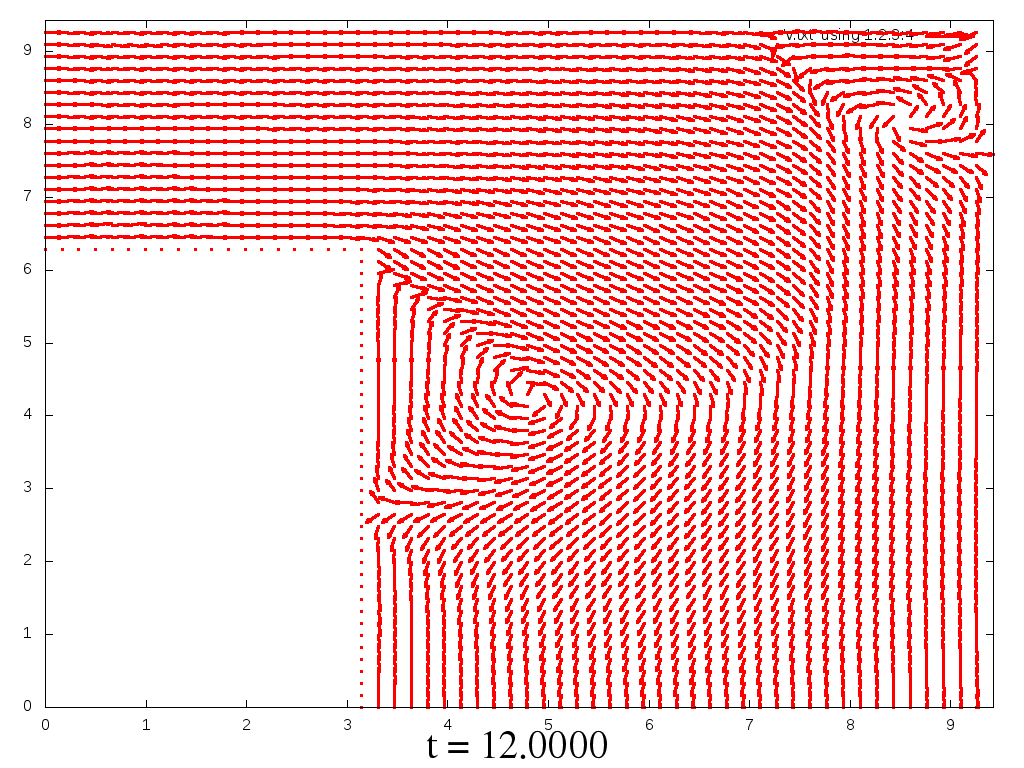
\includegraphics[width=1\linewidth]{./img/01_1_1/V/60}
	\end{minipage}
	\hfill
	\begin{minipage}[h]{0.4\linewidth}
		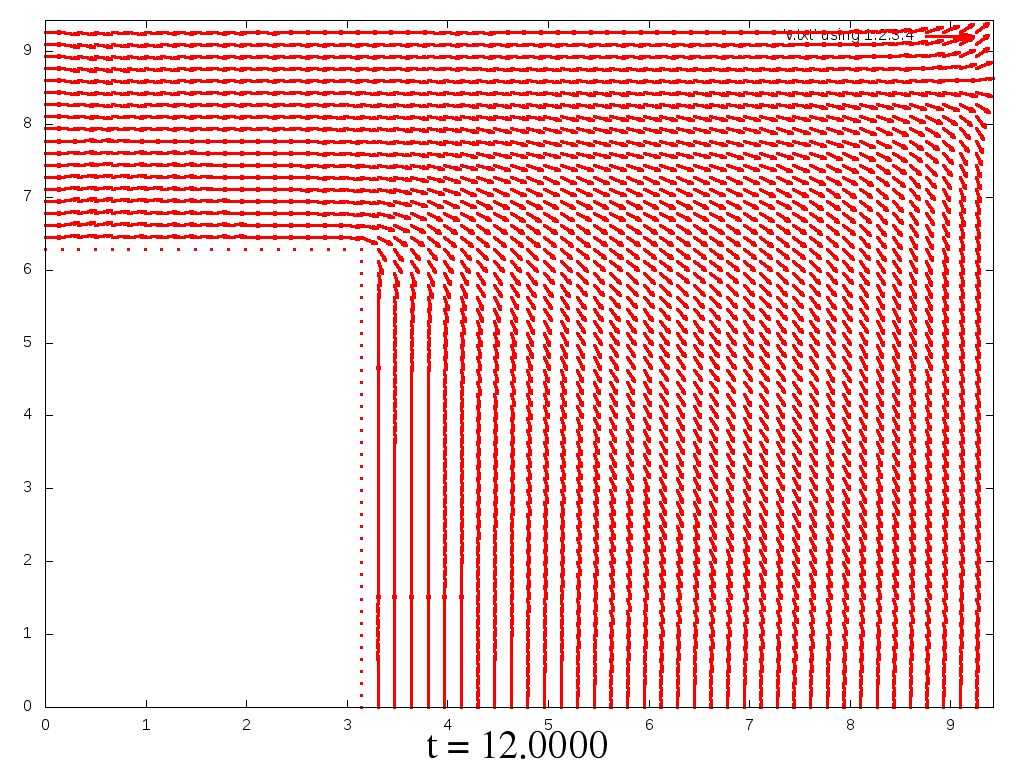
\includegraphics[width=1\linewidth]{./img/01_1_01/V/60}
	\end{minipage}
\end{figure}

\begin{figure}[h]
	\begin{minipage}[h]{0.4\linewidth}
		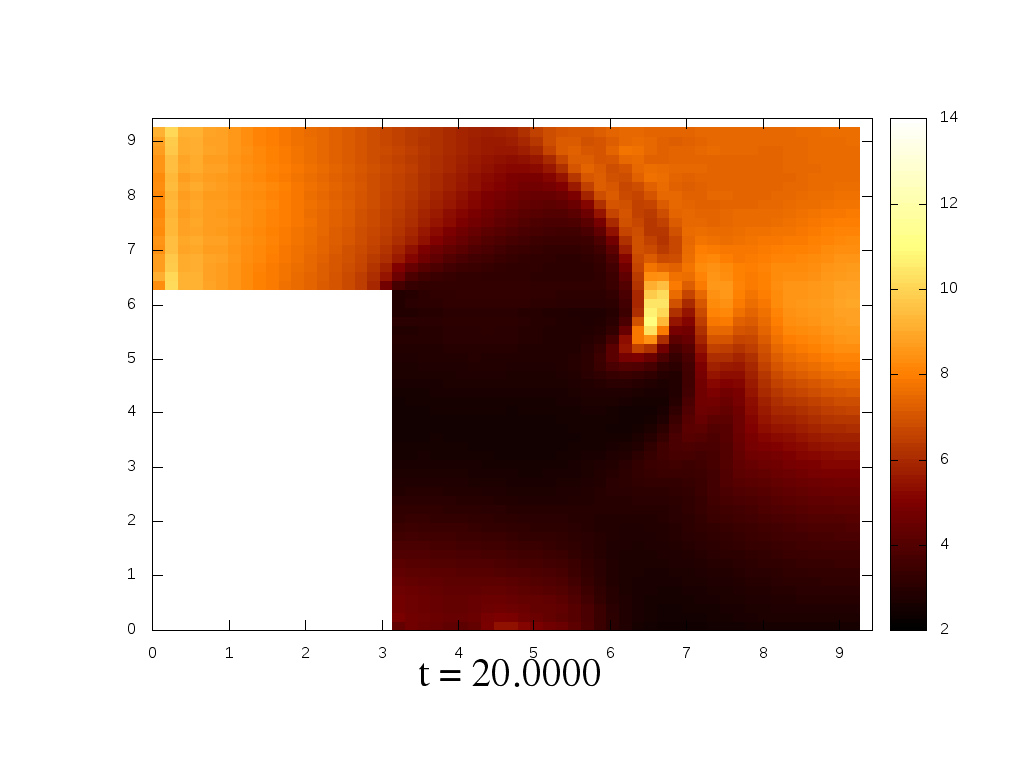
\includegraphics[width=1\linewidth]{./img/01_1_1/G/100}
	\end{minipage}
	\hfill
	\begin{minipage}[h]{0.4\linewidth}
		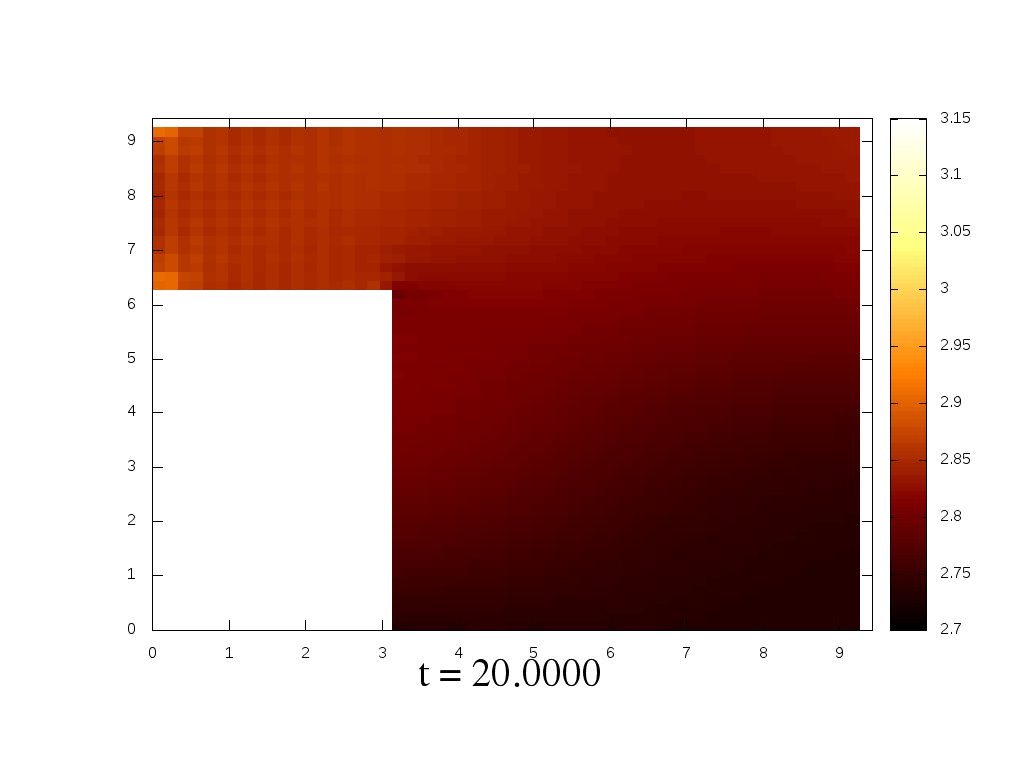
\includegraphics[width=1\linewidth]{./img/01_1_01/G/100}
	\end{minipage}
\end{figure}
\begin{figure}[h]
\begin{minipage}[h]{0.4\linewidth}
	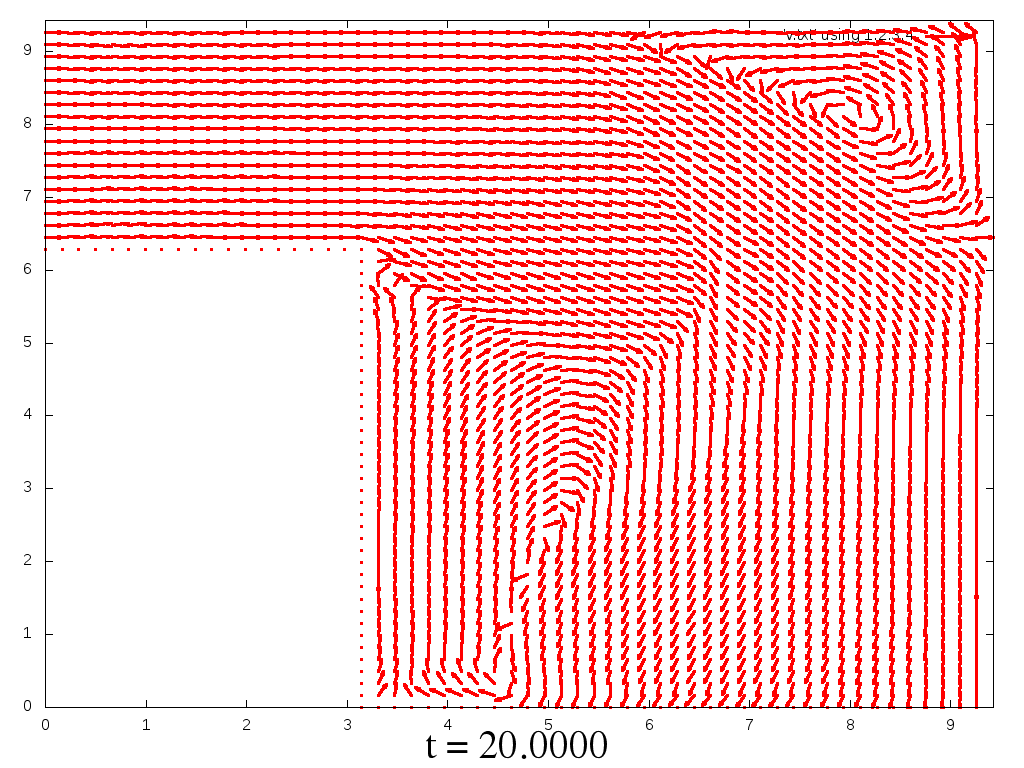
\includegraphics[width=1\linewidth]{./img/01_1_1/V/100}
\end{minipage}
\hfill
\begin{minipage}[h]{0.4\linewidth}
	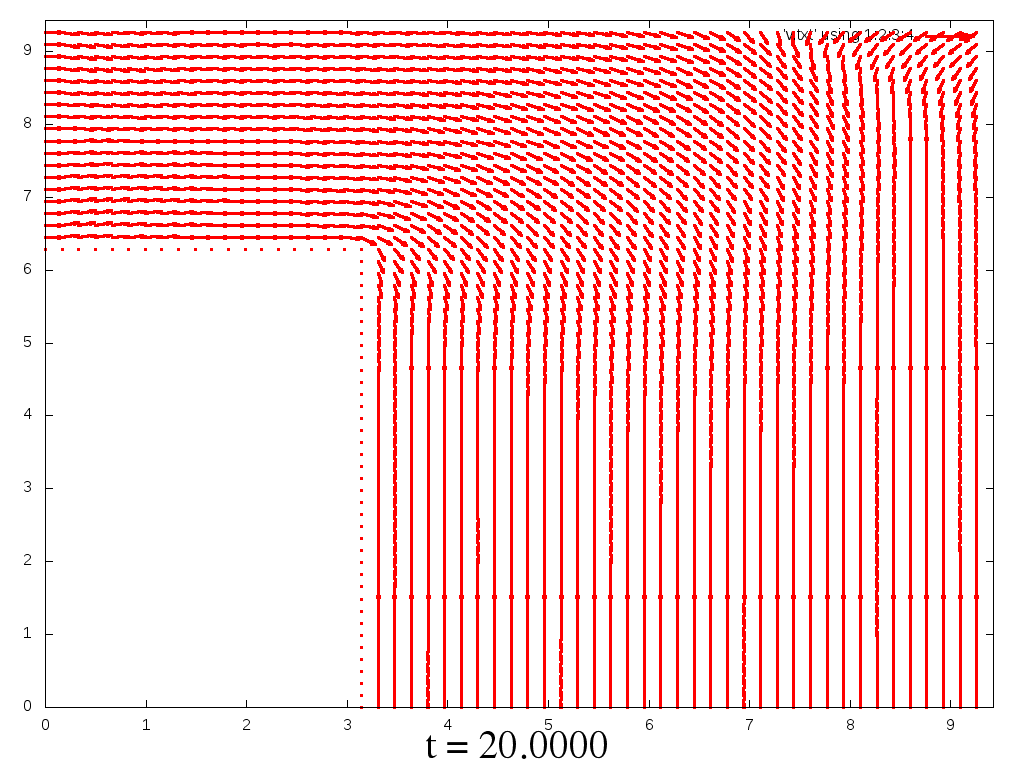
\includegraphics[width=1\linewidth]{./img/01_1_01/V/100}
\end{minipage}
\end{figure}

\begin{figure}[h]
	\begin{minipage}[h]{0.4\linewidth}
		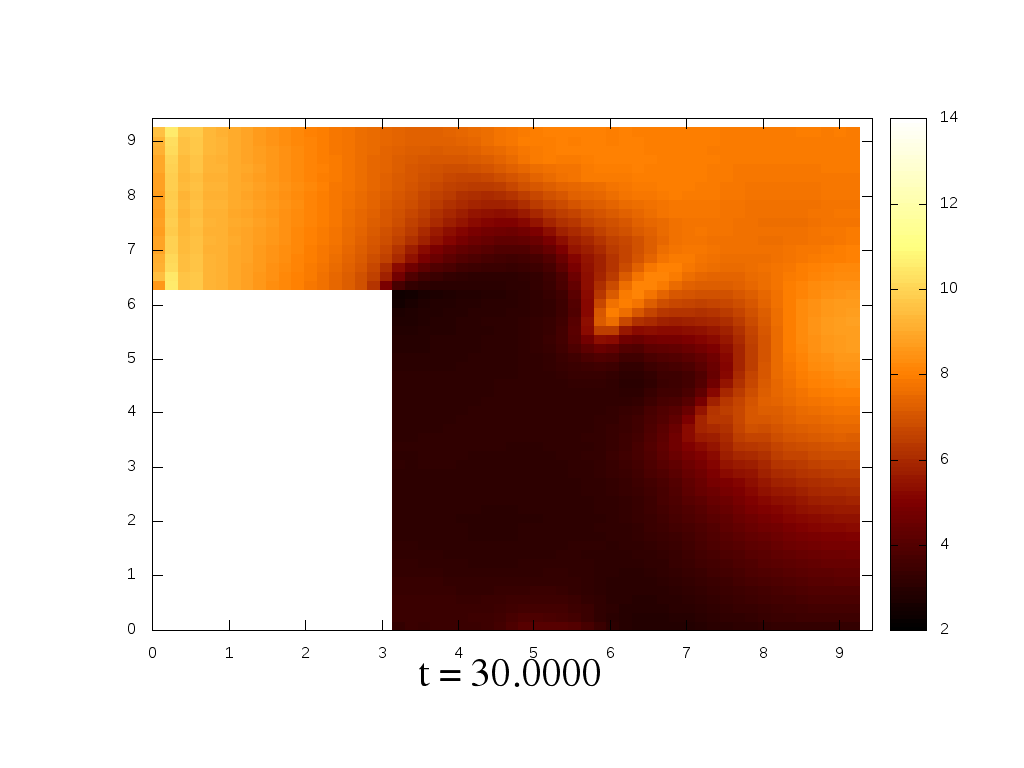
\includegraphics[width=1\linewidth]{./img/01_1_1/G/150}
	\end{minipage}
	\hfill
	\begin{minipage}[h]{0.4\linewidth}
		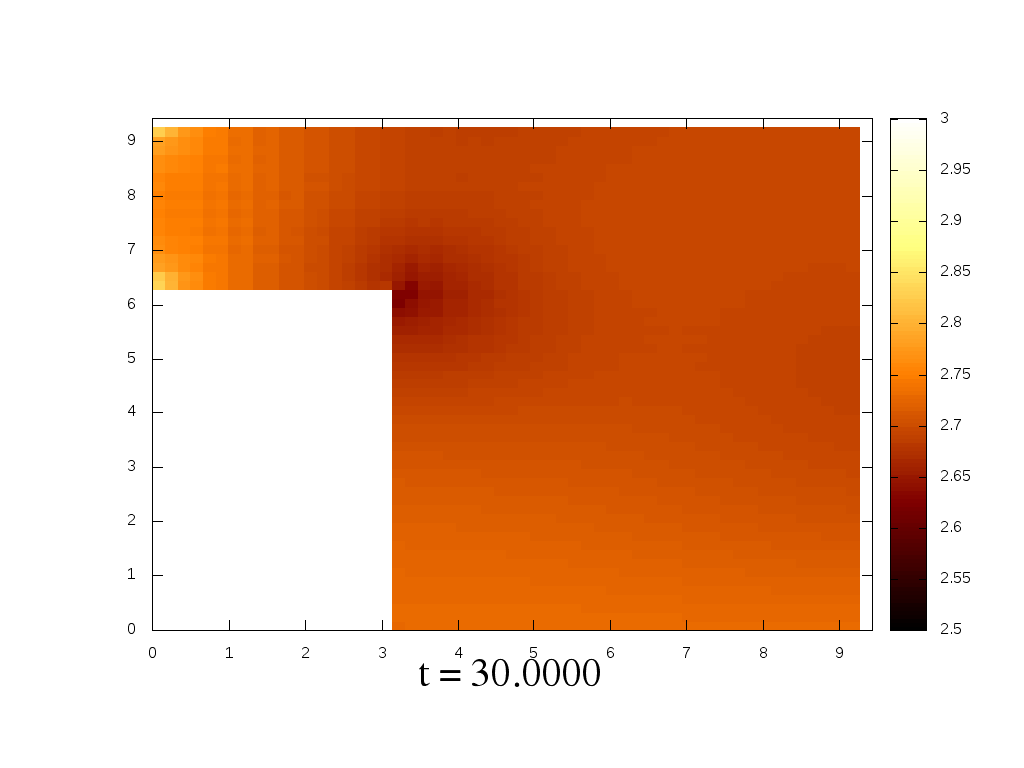
\includegraphics[width=1\linewidth]{./img/01_1_01/G/150}
	\end{minipage}
\end{figure}

\begin{figure}[h]
\begin{minipage}[h]{0.4\linewidth}
	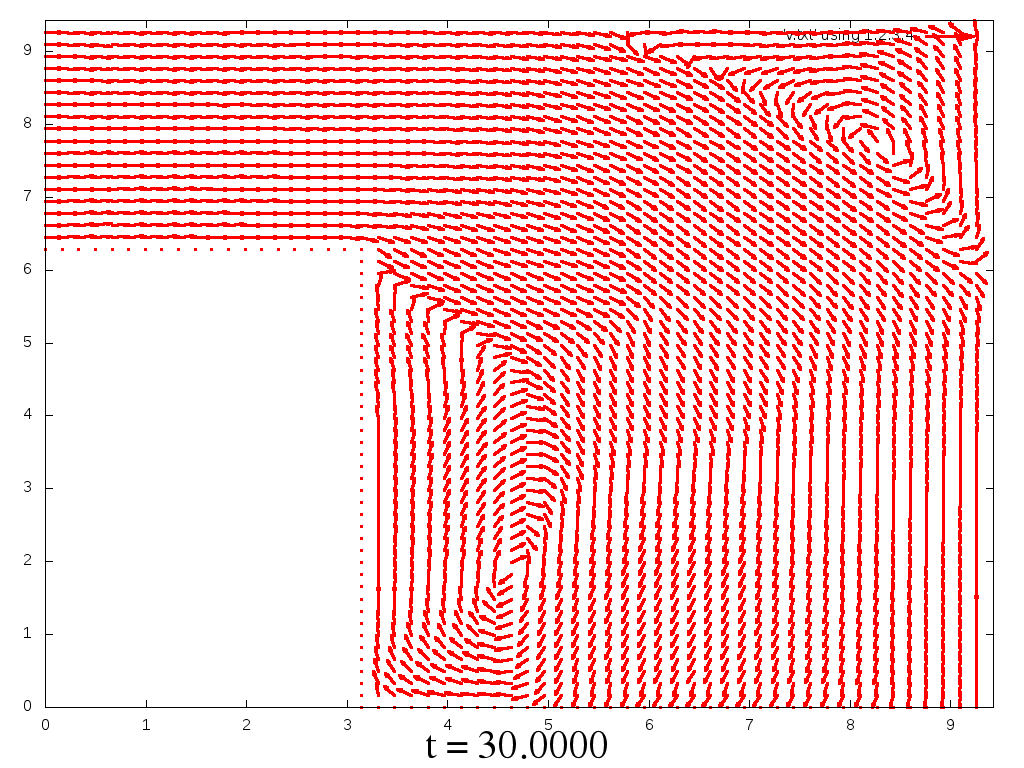
\includegraphics[width=1\linewidth]{./img/01_1_1/V/150}
\end{minipage}
\hfill
\begin{minipage}[h]{0.4\linewidth}
	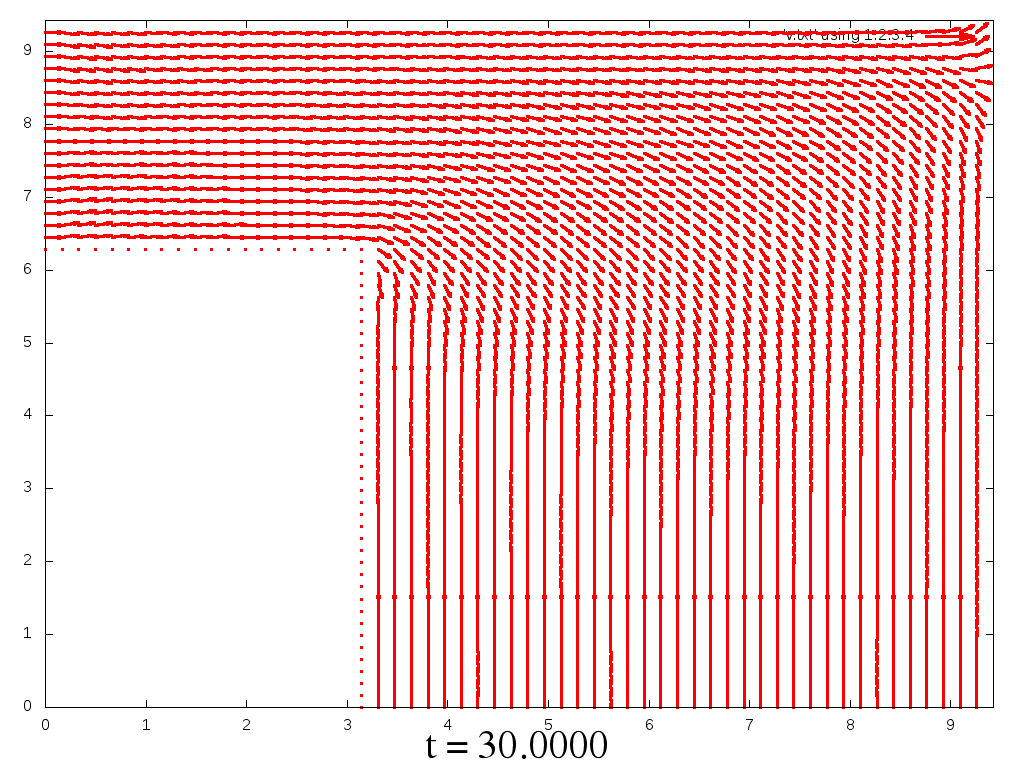
\includegraphics[width=1\linewidth]{./img/01_1_01/V/150}
\end{minipage}
\end{figure}

\begin{figure}[h]
	\begin{minipage}[h]{0.4\linewidth}
		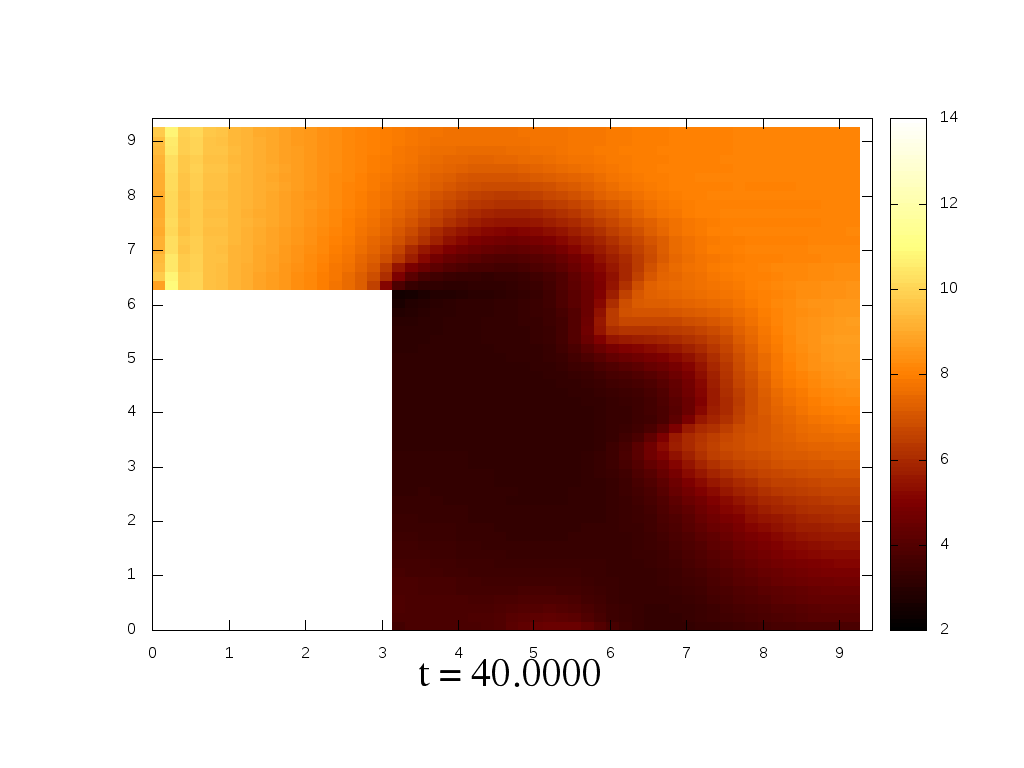
\includegraphics[width=1\linewidth]{./img/01_1_1/G/200}
	\end{minipage}
	\hfill
	\begin{minipage}[h]{0.4\linewidth}
		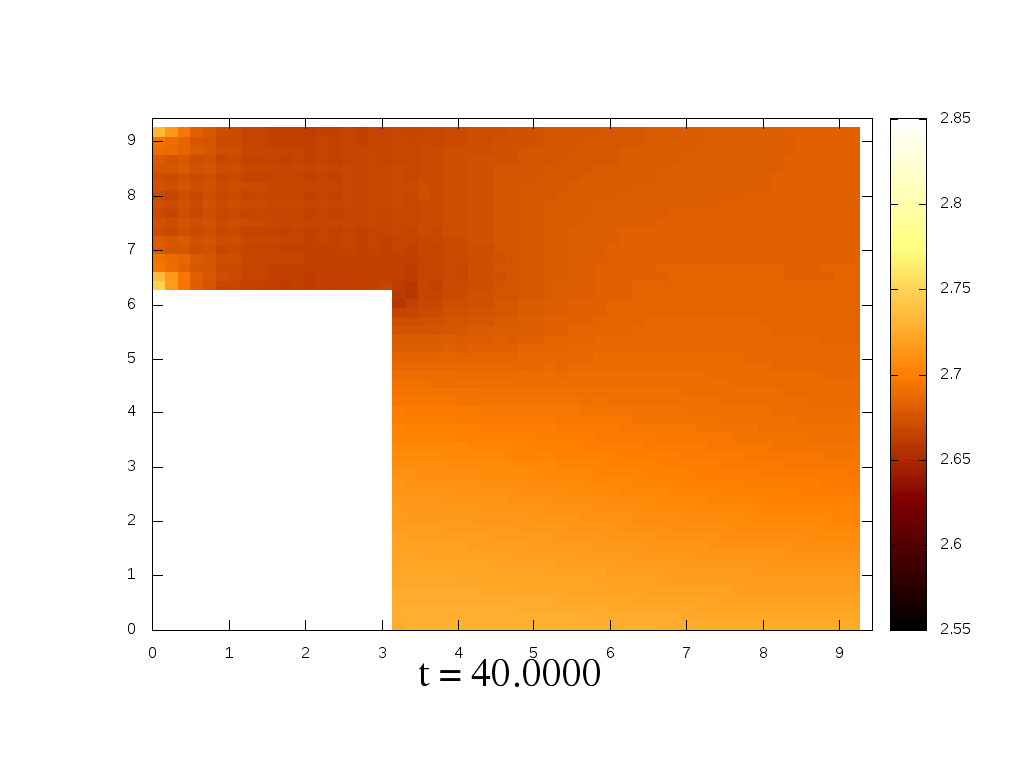
\includegraphics[width=1\linewidth]{./img/01_1_01/G/200}
	\end{minipage}
\end{figure}

\begin{figure}[h]
	\begin{minipage}[h]{0.4\linewidth}
		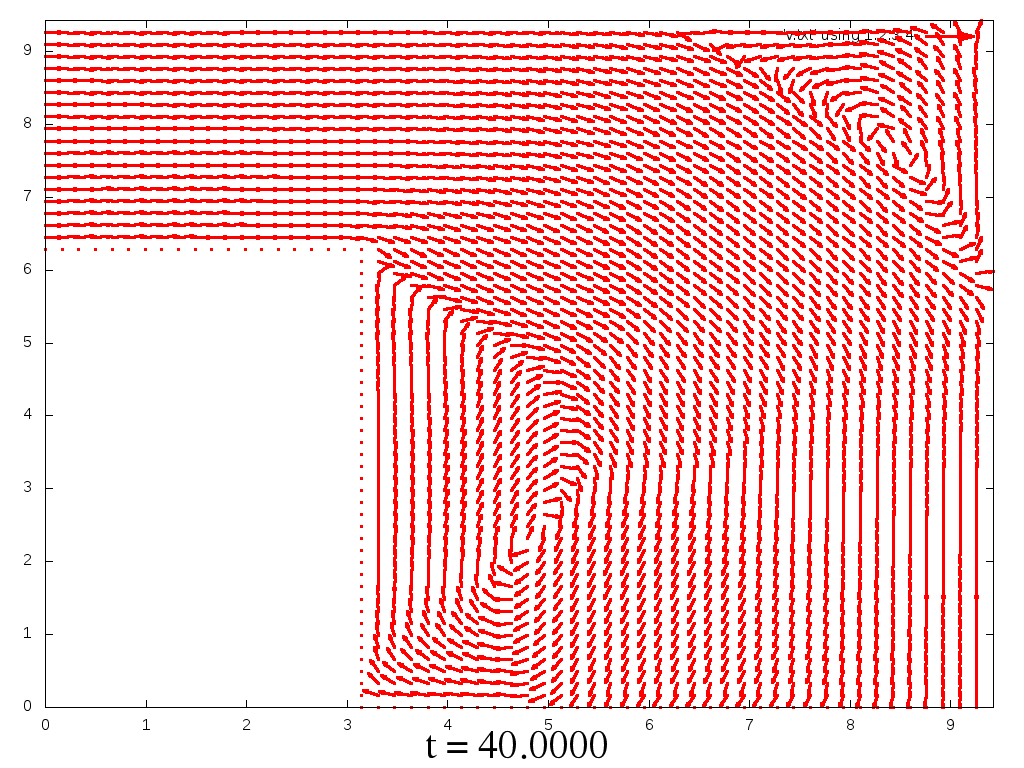
\includegraphics[width=1\linewidth]{./img/01_1_1/V/200}
	\end{minipage}
	\hfill
	\begin{minipage}[h]{0.4\linewidth}
		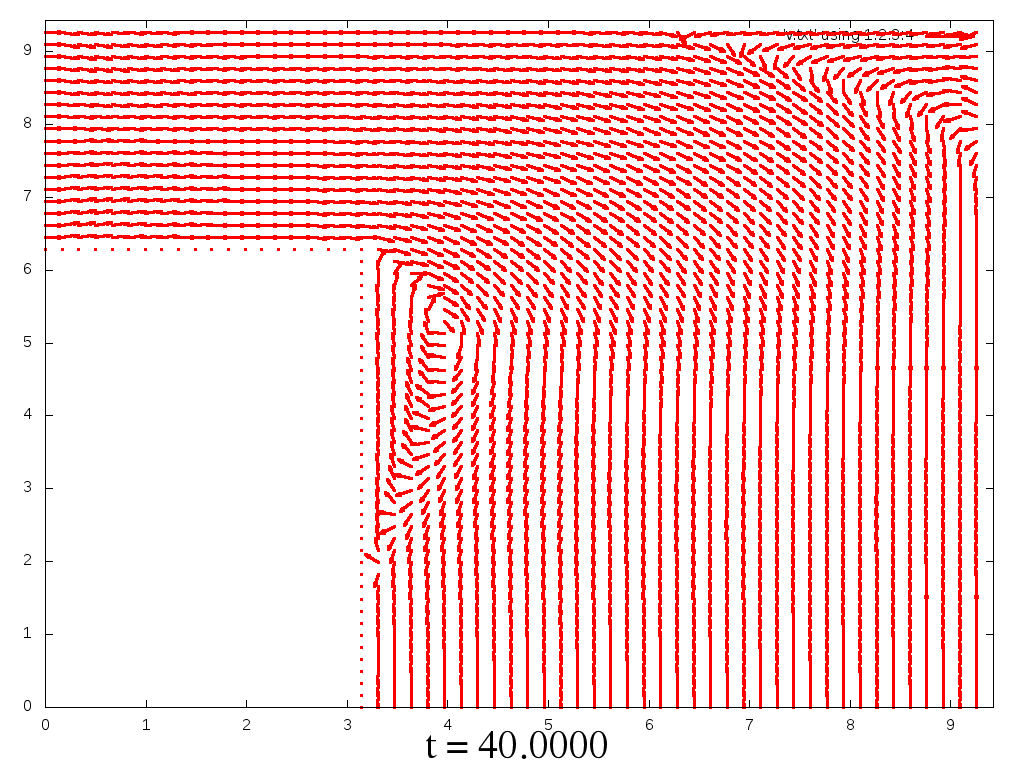
\includegraphics[width=1\linewidth]{./img/01_1_01/V/200}
	\end{minipage}
\end{figure}

На графиках хорошо видно, что при относительно большой скорости возникают вихри.
При относительно маленькой скорости течение газа происходит гладко.





\end {document}
